\documentclass[12pt]{article}
\usepackage{tabularx}
\usepackage{multirow}
\usepackage{makecell}
\usepackage{changepage}
\usepackage{xifthen}
\usepackage{amsmath,amssymb}
\usepackage{setspace}
\usepackage{xcolor}
\usepackage{graphicx,caption}
\usepackage{subcaption}
\usepackage{enumitem}
\usepackage{caption}
\usepackage{array}
\usepackage{booktabs}
\usepackage{hyperref}
\hypersetup{colorlinks=true,linkcolor=blue}
\usepackage{comment}
\usepackage[backend=biber]{biblatex}
\addbibresource{ref.bib}

\parindent 0em
\setcounter{secnumdepth}{3}
\setcounter{tocdepth}{3}

\renewcommand{\baselinestretch}{1.2}
\usepackage[includehead,left=3.25cm,right=2.5cm,top=2.5cm,headsep=1.5cm,headheight=0.0cm,bottom=2.5cm,footskip=1.0cm]{geometry}
\raggedbottom

\title{\textbf{Channel-Aware Cooperative Perception for Blind Spot Detection in V2X Networks}}

\author{Aiden McGarrie, Rageshwaree Beegodhur, Vanessa Vo \\ \textit{School of Electrical Engineering and Computer Science,} \\ \textit{University of Ottawa, Canada}}

\date{}

\begin{document}

\maketitle

\begin{abstract}
\noindent
Autonomous vehicles have become a focal point of research and development because of their ability to perceive their surroundings. However, physical obstructions and limited perceptions create blind spots onboard sensors cannot resolve alone. This report proposes a channel-aware cooperative vehicle-infrastructure perception system that addresses this issue by using a Roadside Unit (RSU) to detect objects in blind spots and selectively transmit the information to nearby vehicles using a bandwidth-constrained Vehicle-to-Everything (V2X) channel.

\medskip
\noindent
The system operates as an end-to-end pipeline on the DAIR-V2X dataset, combining YOLOv10-N object detection, ByteTrack multi-object tracking, and bird's eye view localization using monocular depth and LiDAR calibration. A Hungarian matching algorithm with a depth-aware Mahalanobis distance cost matrix identifies blind spot targets, and a lightweight Multi-Layer Perceptron (MLP) Semantic Gate prioritizes which targets to transmit under realistic per-frame bandwidth budgets.

\medskip
\noindent
Comparative testing demonstrates the MLP Semantic Gate consistently outperforms Hard Gate, No Gate, and Random baselines across all transmission levels, achieving a precision-recall score of 0.551 compared to a random baseline of 0.023. The results highlight that prioritizing bandwidth meaningfully improves cooperative perception under real-world communication constraints.
\end{abstract}

\newpage
\tableofcontents
\newpage

\section{Introduction}

A car moving through a busy intersection sees only what its cameras and sensors can reach. Anything blocked by another vehicle, a building, or a roadside structure simply does not exist from its perspective until, often, it is too late. Blind spots are a leading factor in urban collisions, and no amount of sensor improvement on a single vehicle fully solves the problem. The physics of line-of-sight means something will always be hidden.

\medskip
One practical answer is to stop relying solely on what the vehicle itself can see. RSUs, cameras and sensors mounted at intersections above the flow of traffic, have a fundamentally different vantage point. They can see around corners, over the tops of trucks, and into the gaps between vehicles. If an RSU can communicate what it sees to a nearby vehicle in real time, that vehicle gains awareness it could not produce on its own. This is the core idea behind V2X cooperative perception.

\medskip
The hard part is not the sensing but the communication. A V2X channel has limited bandwidth, and an RSU watching a busy intersection may detect thirty or forty objects per frame. Sending all of them is not realistic. What gets transmitted has to be chosen carefully, and quickly. A system that picks randomly, or sends everything regardless of what the vehicle already knows, wastes the channel on information that does not help. The question is how to identify which detections are actually in the vehicle's blind spot, and then how to rank them when only a few can be sent.

\medskip
This paper describes a system built to answer that question. Using the DAIR-V2X dataset \cite{yu2022dairv2x}, we built a full pipeline that runs detection with YOLOv10-N \cite{wang2024yolov10}, tracks objects over time with ByteTrack \cite{zhang2022bytetrack}, converts detections into shared world coordinates, matches RSU and vehicle object lists to find what the vehicle is missing, and then uses a trained MLP to decide what is worth transmitting given the available bandwidth. The matching step uses Mahalanobis distance rather than simple Euclidean distance, which matters because position uncertainty grows with depth and a naive distance metric ignores that entirely.

\medskip
The contributions of this work are:
\begin{itemize}
    \item A complete cooperative perception pipeline running on real DAIR-V2X data, from raw frames to identified blind spot targets.
    \item A depth-aware covariance model for bird's eye view matching that accounts for how uncertainty scales with distance.
    \item A channel-aware MLP Semantic Gate trained to prioritize true blind spot targets under five different bandwidth levels (L0--L4).
    \item An evaluation comparing MLP, Hard Gate, No Gate, and Random strategies using mAP at 2m, 4m, and 6m thresholds, alongside recall and precision-recall metrics.
\end{itemize}

\section{Related Work}
\label{sec:related}

\subsection{Cooperative Perception and V2X Communication}

The idea of sharing perception data between vehicles is not new, but making it work under real communication constraints has proven difficult. Early V2V work like V2VNet \cite{wang2020v2vnet} showed that sharing intermediate feature maps between vehicles could substantially improve joint state prediction compared to acting on local data alone. The results were compelling, but the approach assumed essentially unlimited communication: every vehicle shared everything with every other vehicle in range. That assumption does not hold in practice.

\medskip
Where2comm \cite{hu2022where2comm} was one of the first systems to treat bandwidth as a hard constraint rather than an afterthought. It used spatial confidence maps to identify which parts of the scene were actually informative and transmitted only those regions, cutting communication volume significantly while preserving most of the accuracy gain. More recent work on task-oriented semantic communication \cite{gan2026scomcp} takes this further, asking not just which features are informative but which are relevant to the specific downstream task. Our approach follows a similar philosophy: rather than compressing or filtering raw features, we train a small classifier to score each blind spot candidate by how much it matters to the receiving vehicle, then transmit only the top-ranked ones.

\subsection{Object Detection}

Object detection sits at the foundation of every perception pipeline we are aware of. The field split early into two camps. Two-stage detectors like Faster R-CNN \cite{ren2016faster} propose candidate regions first and then classify them, which gives strong accuracy but at a speed cost that makes real-time deployment difficult. Single-stage detectors like You Only Look Once (YOLO) \cite{redmon2016yolo} collapsed this into one pass over the image, trading some accuracy for a large gain in speed. That tradeoff has narrowed considerably over the years as single-stage methods matured.

\medskip
YOLOv10 \cite{wang2024yolov10} is the detection model used in this work. It removes the need for non-maximum suppression at inference time by using a dual-label assignment strategy during training, which simplifies the pipeline and improves end-to-end speed. The Nano variant, YOLOv10-N, is the smallest member of the family and is specifically intended for hardware with limited compute which is a realistic constraint for an RSU running at the edge.

\subsection{Multi-Object Tracking}

Detection alone gives you a list of boxes per frame with no memory across time. Tracking connects those boxes into trajectories, assigning consistent identities so that the same vehicle keeps the same ID across hundreds of frames. ByteTrack \cite{zhang2022bytetrack} does this by matching not just high-confidence detections but also low-confidence ones that prior methods simply discarded. The reasoning is straightforward: a partially occluded vehicle may generate a weak detection, but it is still the same vehicle and losing track of it causes problems downstream. ByteTrack's two-stage matching keeps these weak detections alive, which meaningfully reduces the number of identity switches in crowded scenes,  exactly the conditions our pipeline operates in.

\subsection{Probabilistic Matching and Mahalanobis Distance}

When you project a camera detection into world coordinates, the resulting position is not a point, it is a distribution. Monocular depth estimation introduces error that grows as distance increases, and that error is not symmetric: longitudinal uncertainty (how far away something is) grows much faster than lateral uncertainty (how far left or right it is). A matching algorithm that treats each detection as a precise point and measures Euclidean distance between them ignores all of this, leading to false matches at range and missed matches near the camera where everything is crowded together.

\medskip
The Mahalanobis distance \cite{mahalanobis1936} addresses this by folding the covariance structure of each detection's uncertainty directly into the distance calculation. Two detections that are far apart in meters but within each other's uncertainty ellipses will have a small Mahalanobis distance; two detections that are close in meters but with very different uncertainty structures will have a larger one. Paired with the Hungarian algorithm \cite{kuhn1955hungarian} for optimal one-to-one assignment, this gives a matching framework that is substantially more robust to the noise inherent in real-world BEV projections.

\section{Methodology}
\label{sec:method}

\subsection{Dataset}

All experiments in this paper use the DAIR-V2X Cooperative dataset \cite{yu2022dairv2x}, recorded in urban China across a range of real intersection scenarios. The dataset pairs a vehicle-mounted camera with a fixed infrastructure RSU camera at the same location, providing synchronized frames from both viewpoints along with LiDAR scans, 3D bounding box annotations, and full sensor calibration for both platforms.

\medskip
There are 8,577 vehicle-side frames and 15,285 infrastructure-side frames in total. Each frame comes with ground-truth 3D labels giving the true world position of every object in the scene, which we use both to generate training labels for the Semantic Gate and to evaluate blind spot detection accuracy at the end. The calibration files provide the extrinsic and intrinsic parameters needed to move detections out of image space and into a shared world coordinate system. Without these, cross-view matching would not be possible.

\medskip
Seven classes are detected throughout: Car, Van, Bus, Truck, Cyclist, Motorcyclist, and Trafficcone. For training the vehicle-side detector we split the data 80/20 into 12,228 training images and 3,057 validation images, using a fixed random seed of 42 so the split is reproducible. DAIR-V2X stores labels as JSON files with pixel-coordinate bounding boxes in \texttt{(xmin, ymin, xmax, ymax)} format; these were converted to YOLO's normalized \texttt{(class\_id, x\_center, y\_center, width, height)} format before training.

\subsection{System Pipeline Overview}

The pipeline runs two streams in parallel: one processing RSU frames, one processing vehicle frames, and merges them at the matching stage. Figure~\ref{fig:pipeline} shows the full flow.

\begin{figure}[htbp]
\centering
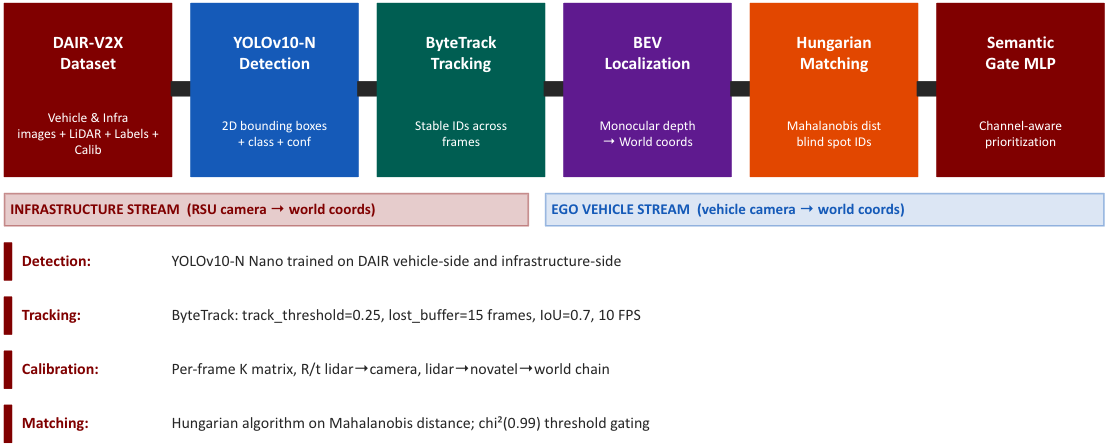
\includegraphics[width=\textwidth]{pipeline_diagram.png}
\caption{System pipeline. Infrastructure and vehicle streams are processed independently through detection, tracking, and BEV localization before being fused at the Hungarian matching stage to identify blind spot targets, which are then ranked by the Semantic Gate MLP for transmission.}
\label{fig:pipeline}
\end{figure}

\medskip
Both streams start with YOLOv10-N producing per-frame detections. ByteTrack then links those detections into tracks with stable IDs. The tracked detections are lifted out of image space into bird's eye view world coordinates using monocular depth and LiDAR calibration data. At the fusion point, the Hungarian algorithm with a Mahalanobis cost matrix matches RSU objects to vehicle objects and anything on the RSU side with no match on the vehicle side is flagged as a blind spot candidate. The Semantic Gate MLP then scores each candidate and selects the top-N to transmit, where N comes from the simulated channel budget.

\subsection{Object Detection Training}

YOLOv10-N was chosen as the detector for both streams. The decision came down to speed and size: as the smallest variant in the YOLOv10 family, it is built for edge deployment on limited hardware, which is a realistic constraint for an RSU running at an intersection. Separate models were trained for the vehicle-side and infrastructure-side cameras since the viewing angles and object appearance differ substantially between the two.

\medskip
\textbf{Training setup.} The vehicle-side model was trained for 150 epochs on an RTX 3070 GPU, taking roughly 8.3 hours. Input resolution was 640$\times$640 with a batch size of 16. We used SGD with a cosine learning rate schedule and standard YOLO data augmentation.

\medskip
\textbf{Results.} Figure~\ref{fig:training_curves} shows the training and validation curves over all 150 epochs. Loss drops consistently across all three components: box, classification, and distribution focal loss on both train and validation sets. There is no visible gap opening between the two, which suggests the model is not overfitting. Precision and recall climb steadily and plateau near the end of training.

\begin{figure}[htbp]
\centering
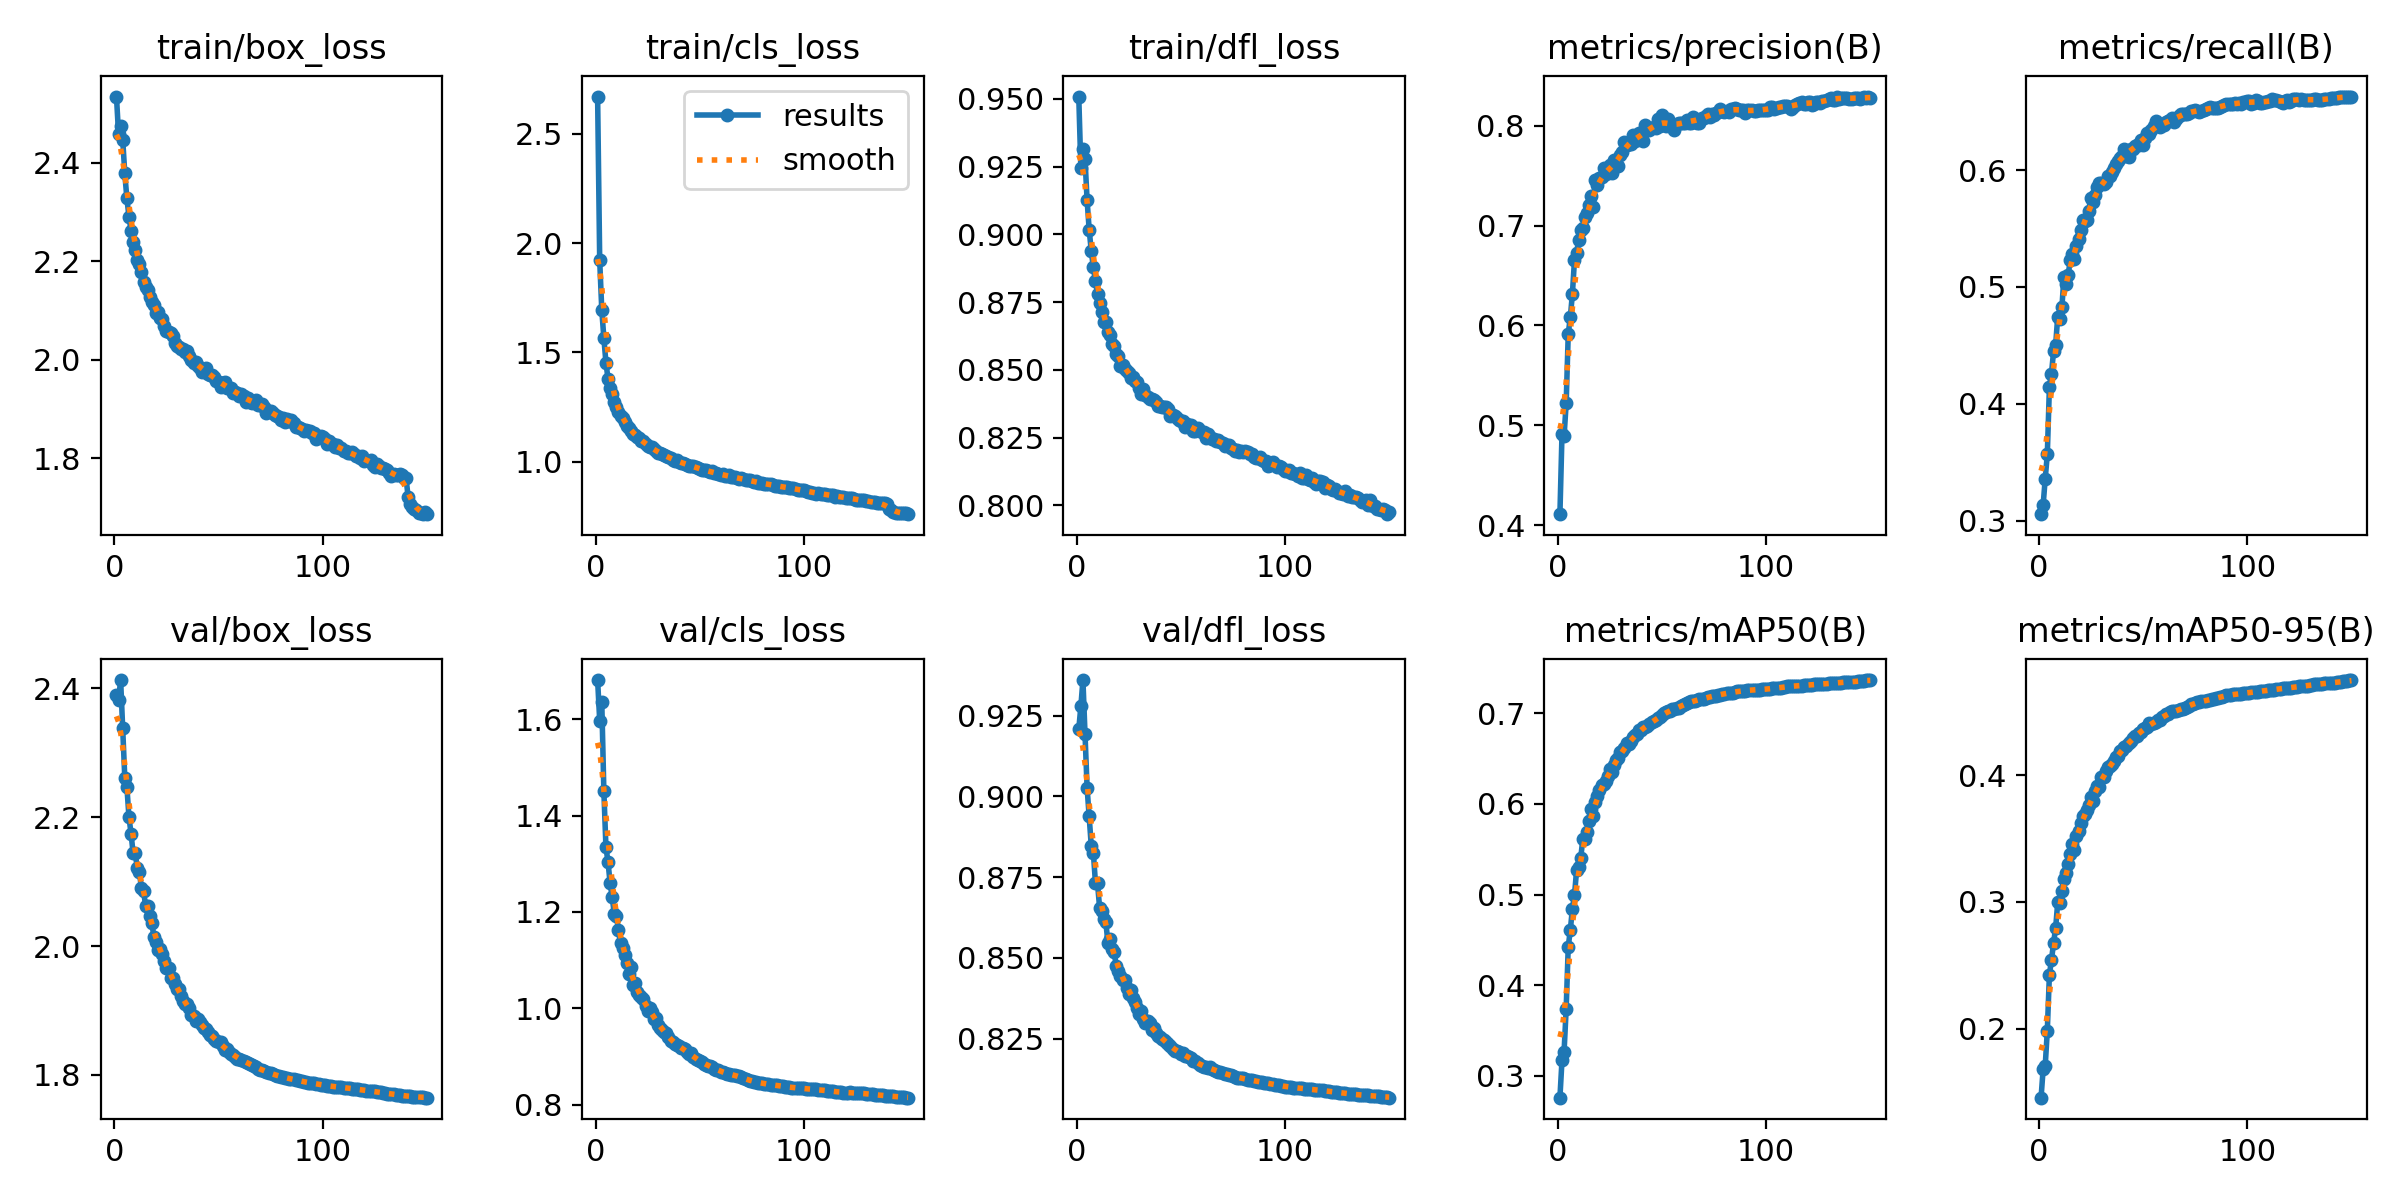
\includegraphics[width=\textwidth]{results.png}
\caption{Training and validation loss curves and validation metrics over 150 epochs for the vehicle-side YOLOv10-N model.}
\label{fig:training_curves}
\end{figure}

\medskip
Final validation metrics at epoch 150 are shown in Table~\ref{tab:detection_results}. The model reaches a precision of 0.828 and recall of 0.663, with mAP@50 of 0.737 and mAP@50-95 of 0.475.

\begin{table}[htbp]
\centering
\caption{Vehicle-side YOLOv10-N validation results at epoch 150.}
\label{tab:detection_results}
\begin{tabular}{lcccc}
\toprule
\textbf{Model} & \textbf{Precision} & \textbf{Recall} & \textbf{mAP@50} & \textbf{mAP@50-95} \\
\midrule
YOLOv10-N (vehicle-side) & 0.828 & 0.663 & 0.737 & 0.475 \\
\bottomrule
\end{tabular}
\end{table}

\medskip
Per-class performance is visible in the Precision-Recall curve in Figure~\ref{fig:pr_curve}. Bus comes out on top at mAP@50 of 0.901, followed by Car at 0.850 and Truck at 0.842. Trafficcone is the weakest at 0.407 because it is small, often partially occluded, and appears far less frequently than cars in the training data, which all work against it. Cyclist and Motorcyclist sit in the middle at 0.669 and 0.703 respectively, reflecting the challenge of detecting smaller, more articulated objects from a forward-facing vehicle camera.

\begin{figure}[htbp]
\centering
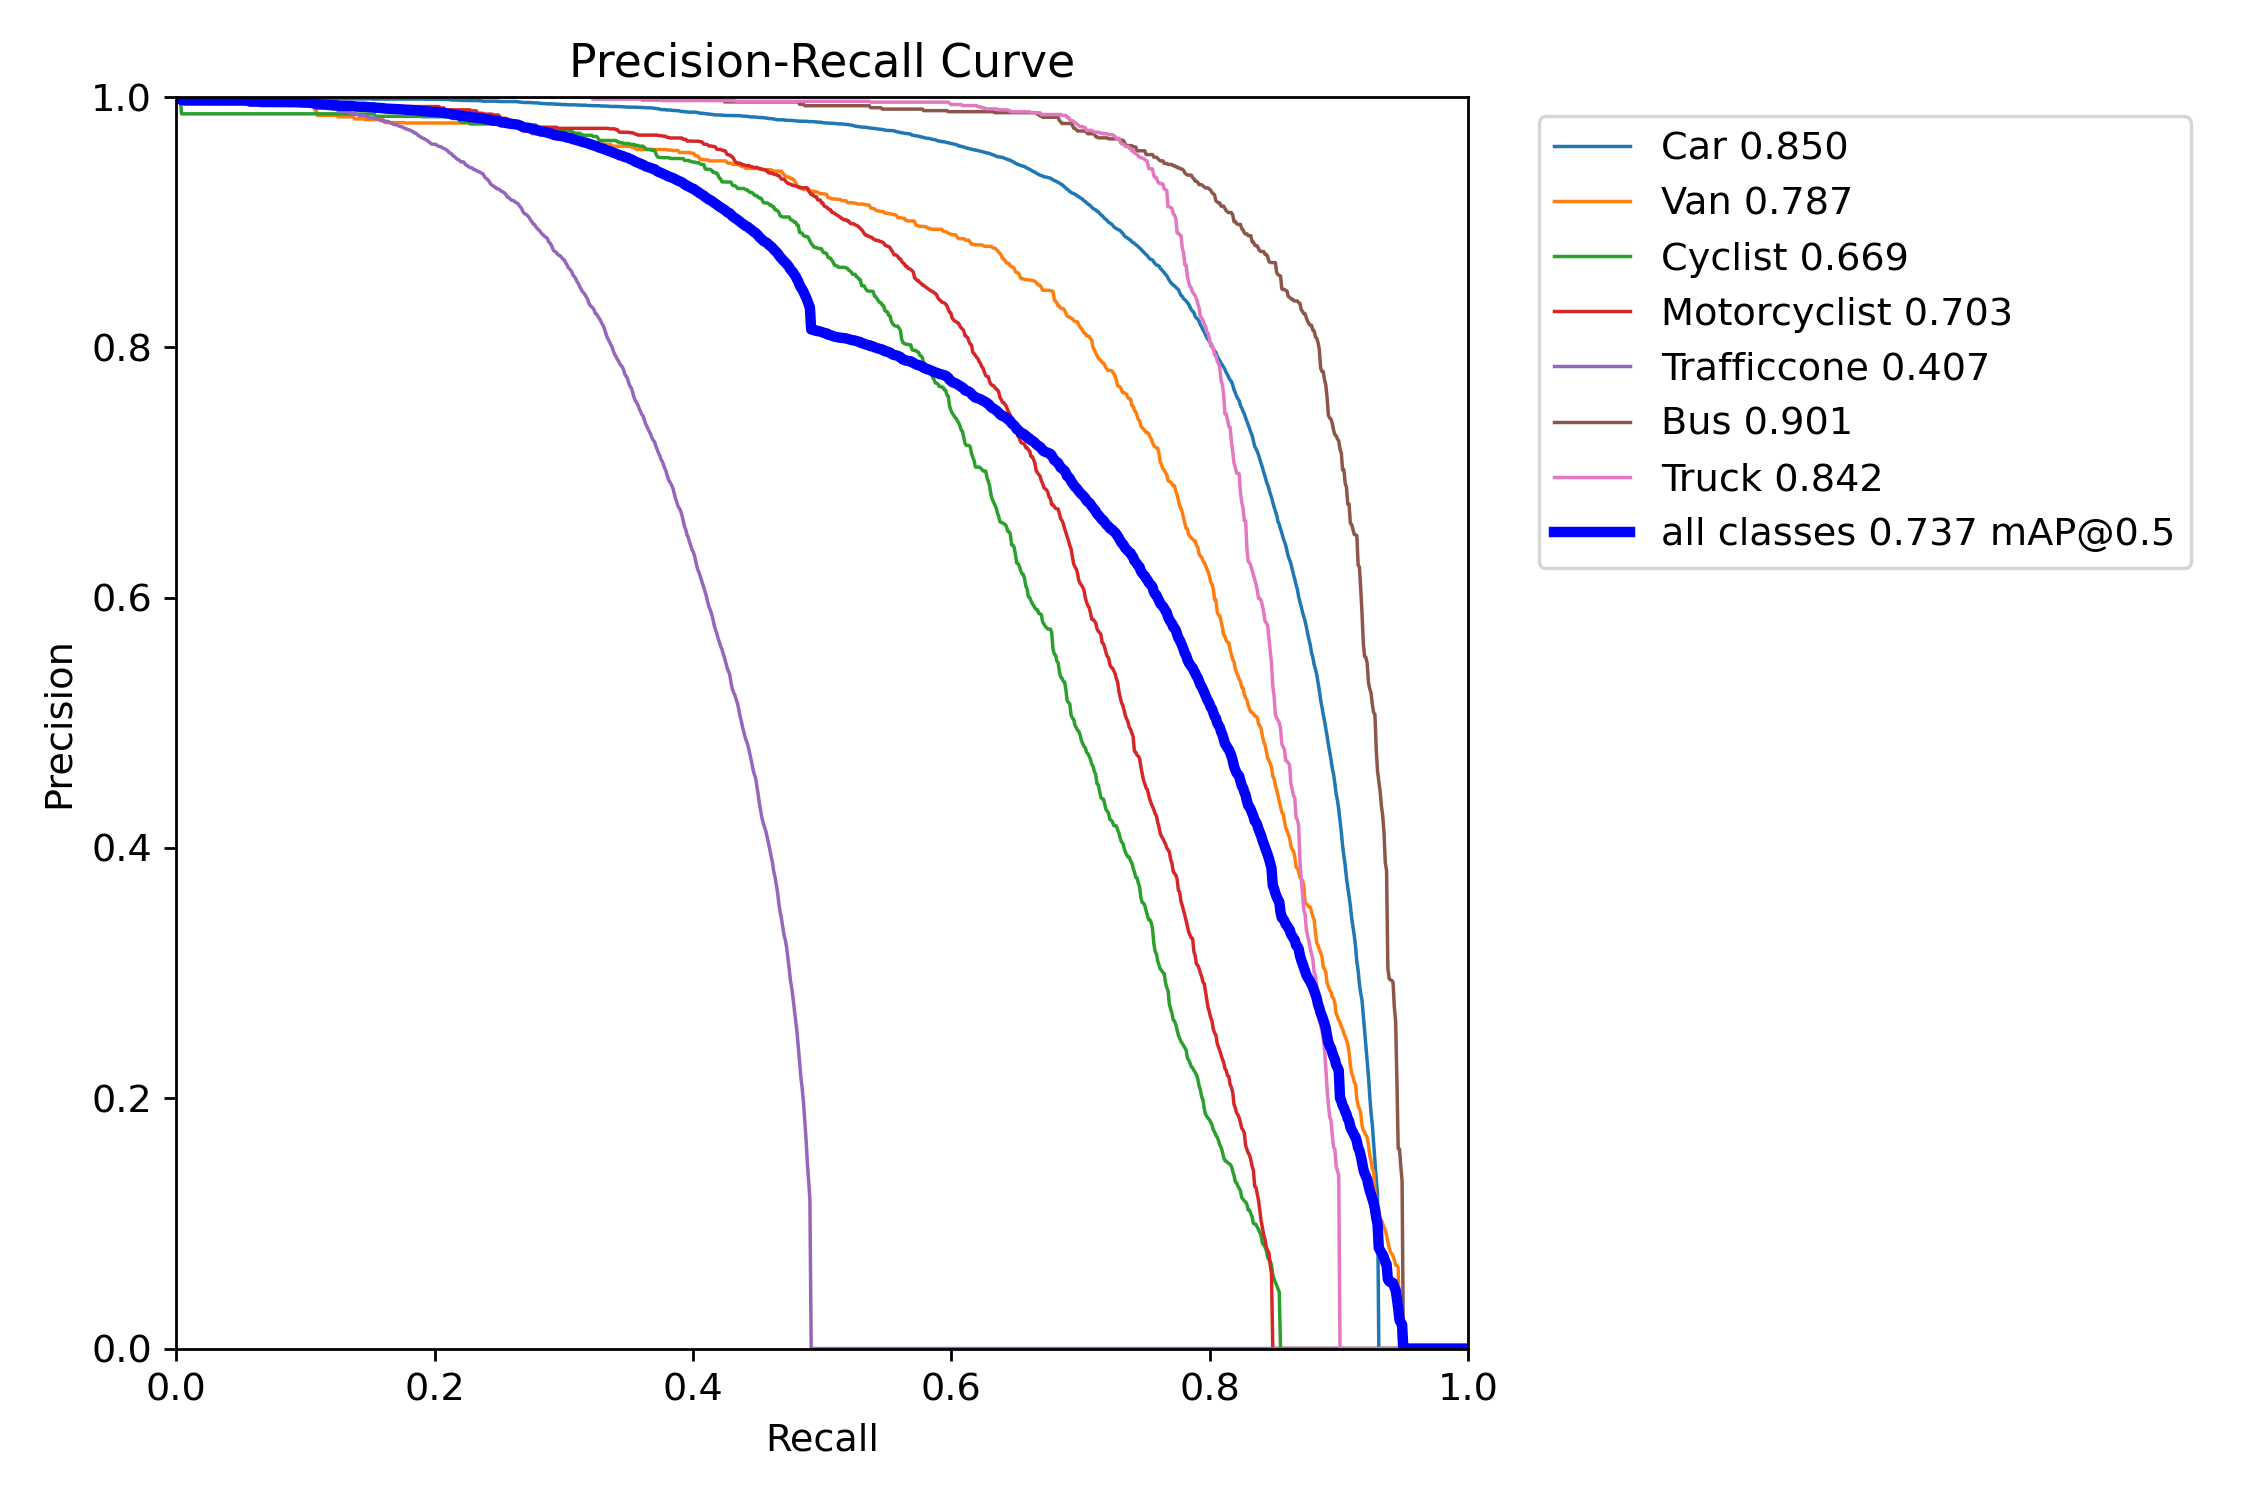
\includegraphics[width=0.75\textwidth]{BoxPR_curve.png}
\caption{Per-class Precision-Recall curves. The bold blue line shows overall mAP@50 of 0.737.}
\label{fig:pr_curve}
\end{figure}

\medskip
The F1-Confidence curve in Figure~\ref{fig:f1_curve} peaks at 0.73 across all classes at a confidence threshold of 0.301. Bus and Truck lead here too, consistent with their stronger mAP scores. The fact that the peak sits at a fairly low confidence threshold reflects the dataset's difficulty. Pushing confidence higher cuts recall faster than it improves precision for most classes.

\begin{figure}[htbp]
\centering
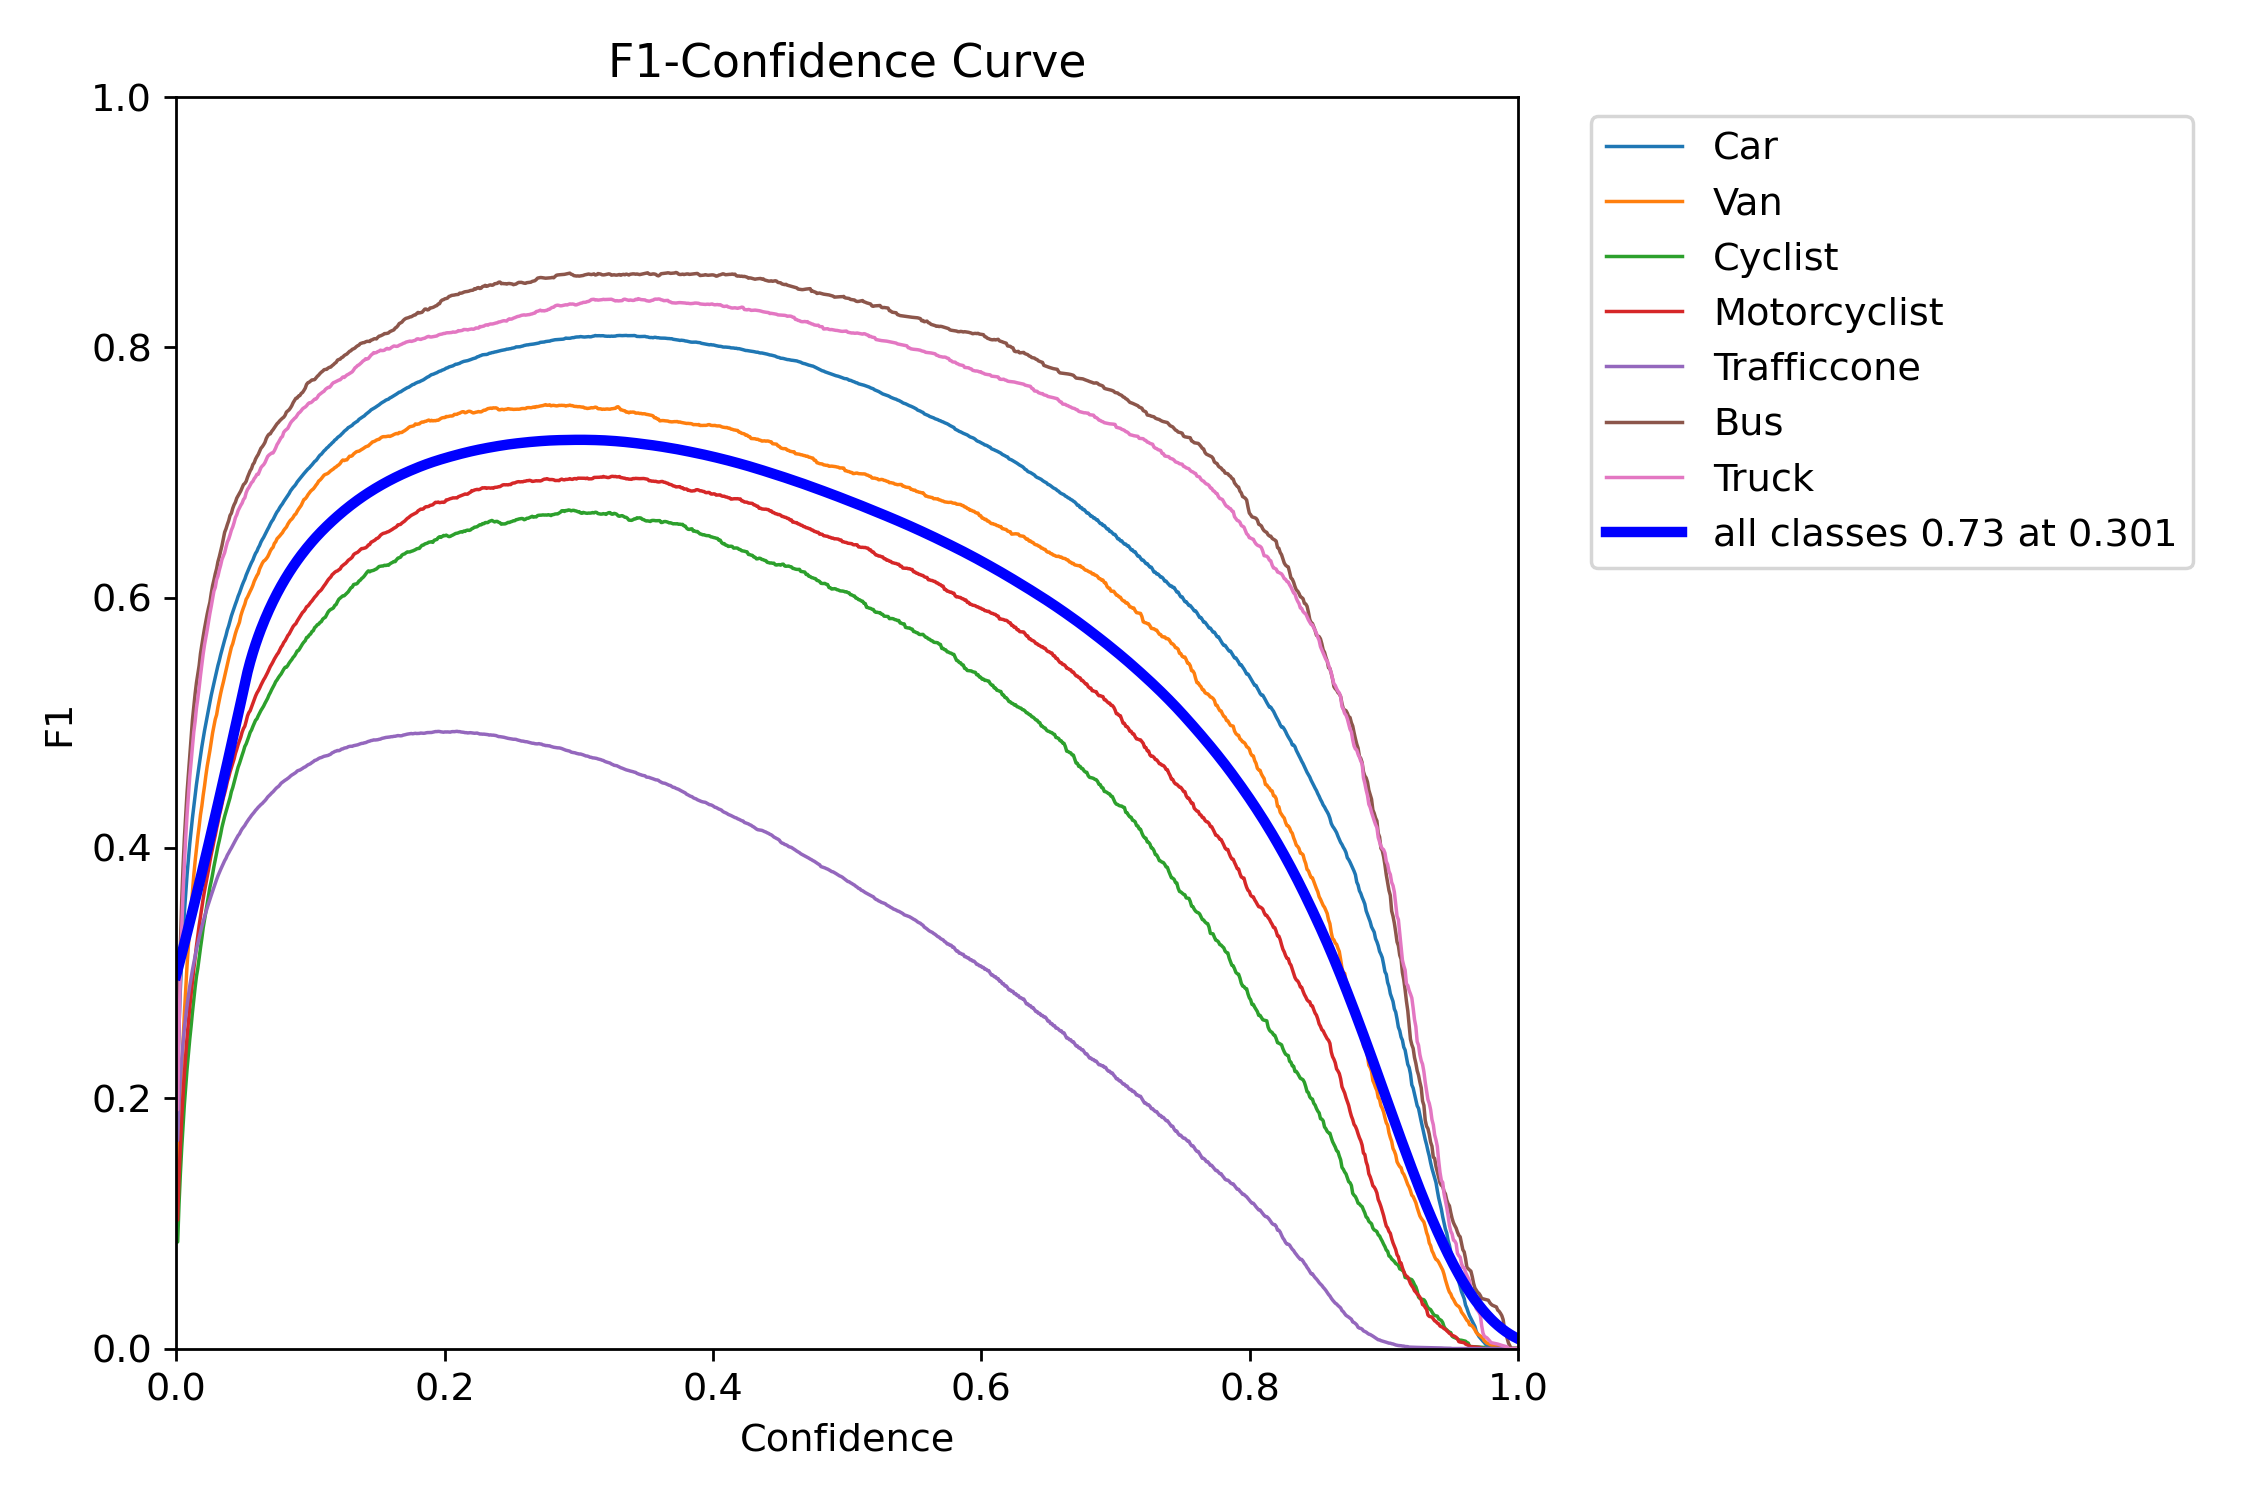
\includegraphics[width=0.75\textwidth]{BoxF1_curve.png}
\caption{F1-Confidence curves per class. Peak all-classes F1 of 0.73 at confidence threshold 0.301.}
\label{fig:f1_curve}
\end{figure}

\medskip
Figure~\ref{fig:confusion} shows the normalized confusion matrix. Bus (0.87) and Car (0.81) are classified most reliably. The main confusion patterns make intuitive sense: 13\% of Cars are called Vans, and 5\% of Motorcyclists are called Cyclists. These pairs look similar from a front-facing camera, particularly at distance. Trafficcone has the worst background confusion rate at 0.62, meaning the model misses it outright most of the time. This is a known challenge with small, thin objects in complex backgrounds.

\begin{figure}[htbp]
\centering
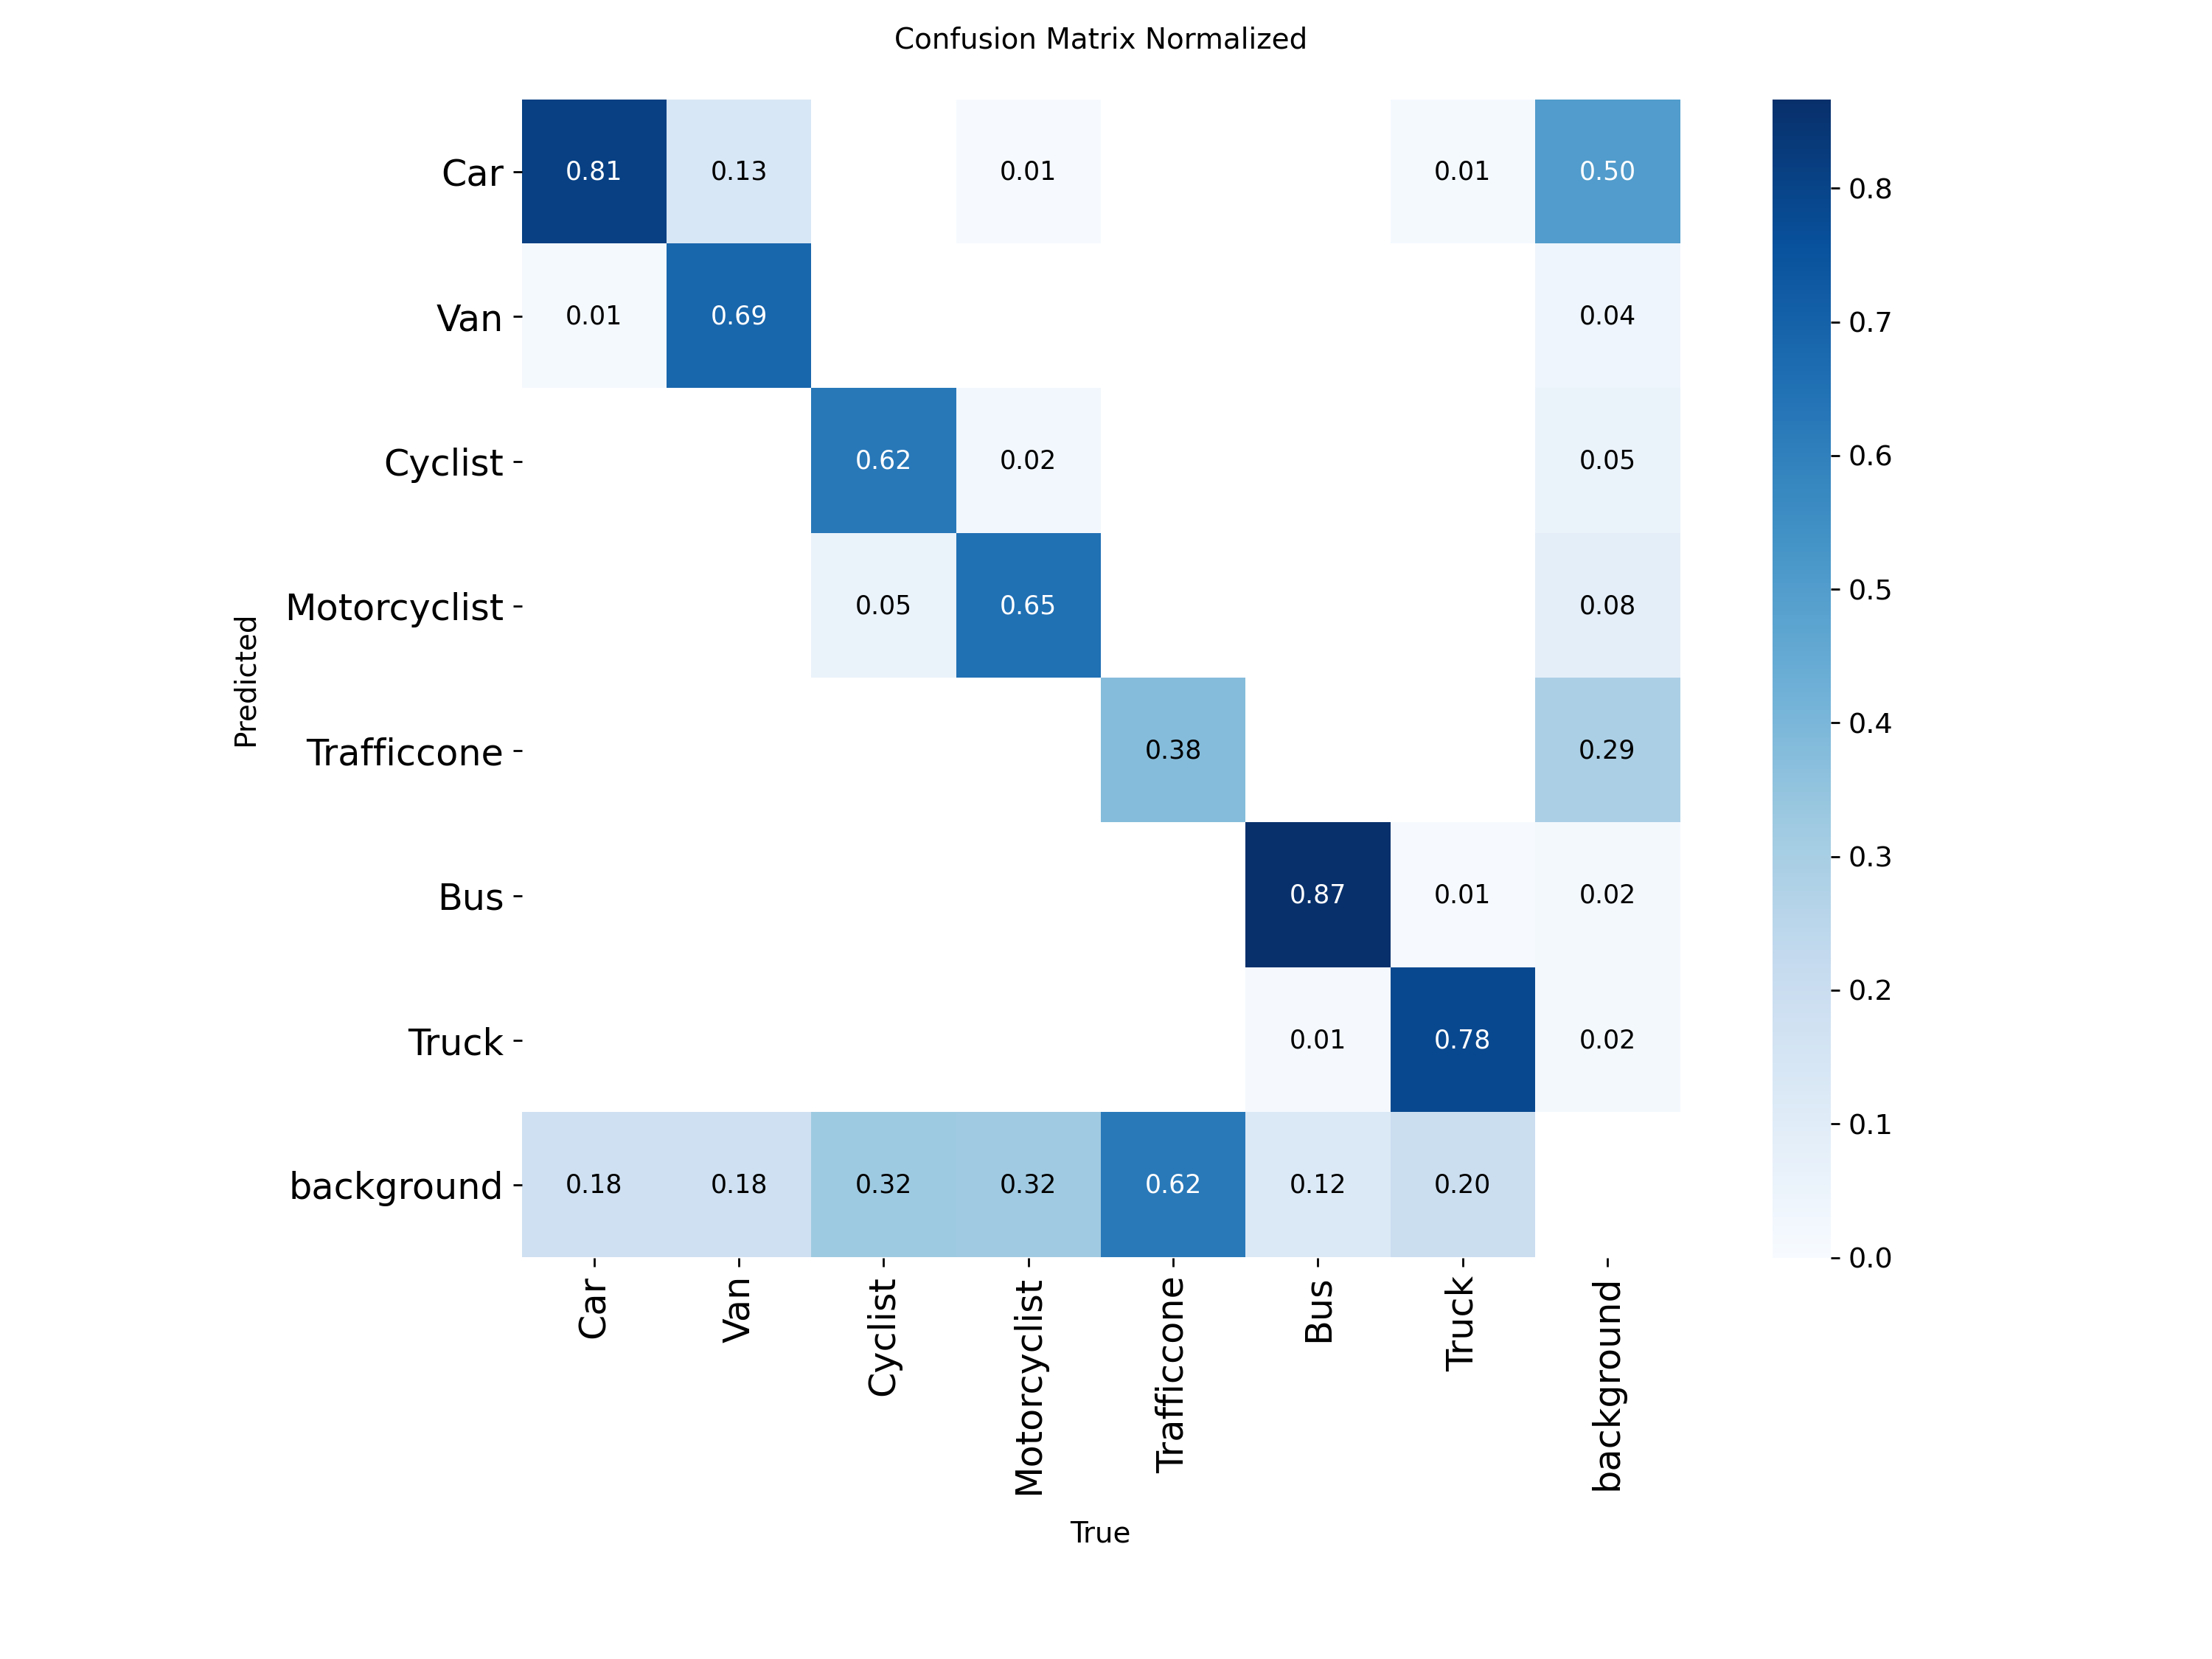
\includegraphics[width=0.75\textwidth]{confusion_matrix_normalized.png}
\caption{Normalized confusion matrix for the vehicle-side YOLOv10-N model on the validation set.}
\label{fig:confusion}
\end{figure}

\medskip
Figure~\ref{fig:val_predictions} shows a sample validation batch with ground truth on the left and model predictions on the right. The model correctly localizes the dominant classes across a range of urban scenes, with the main visible errors occurring on distant or partially occluded objects.

\begin{figure}[htbp]
\centering
\begin{subfigure}[b]{0.48\textwidth}
    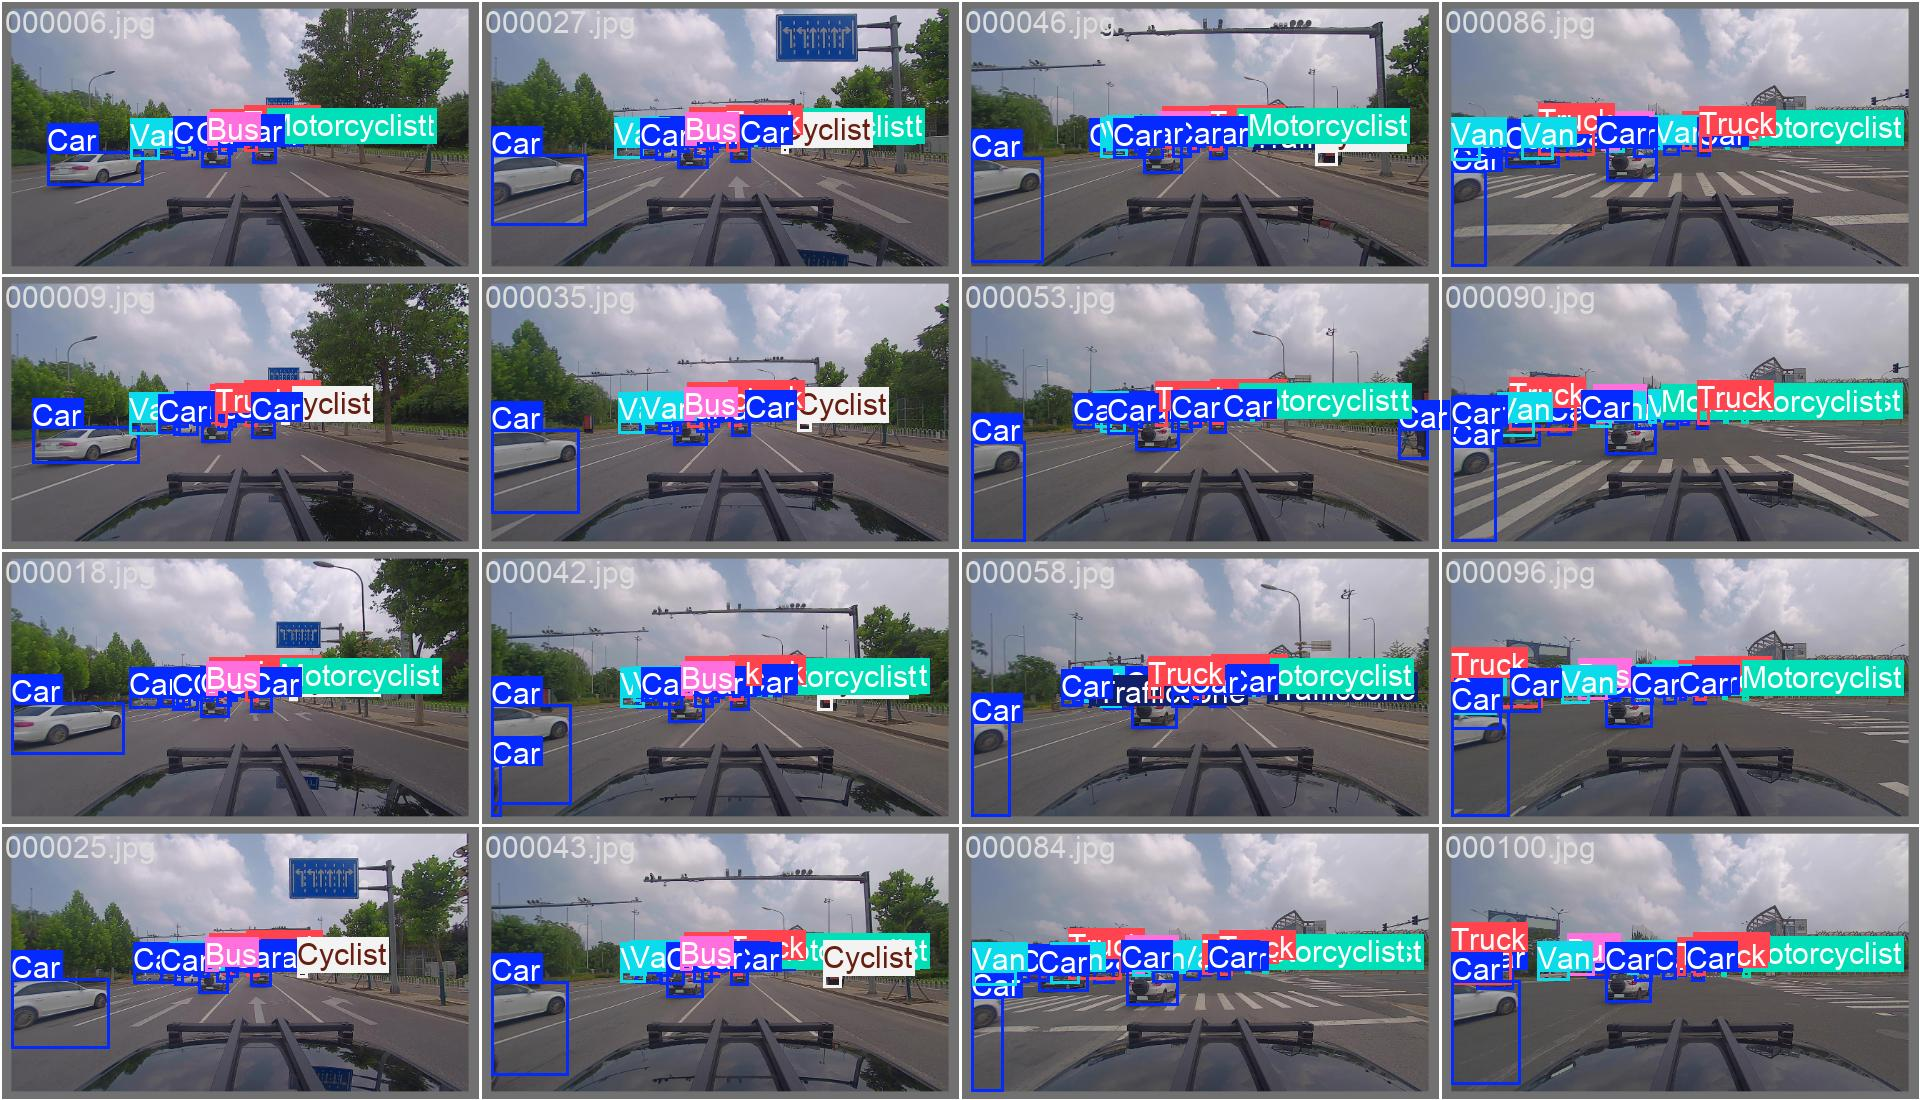
\includegraphics[width=\textwidth]{val_batch0_labels.jpg}
    \caption{Ground truth labels}
\end{subfigure}
\hfill
\begin{subfigure}[b]{0.48\textwidth}
    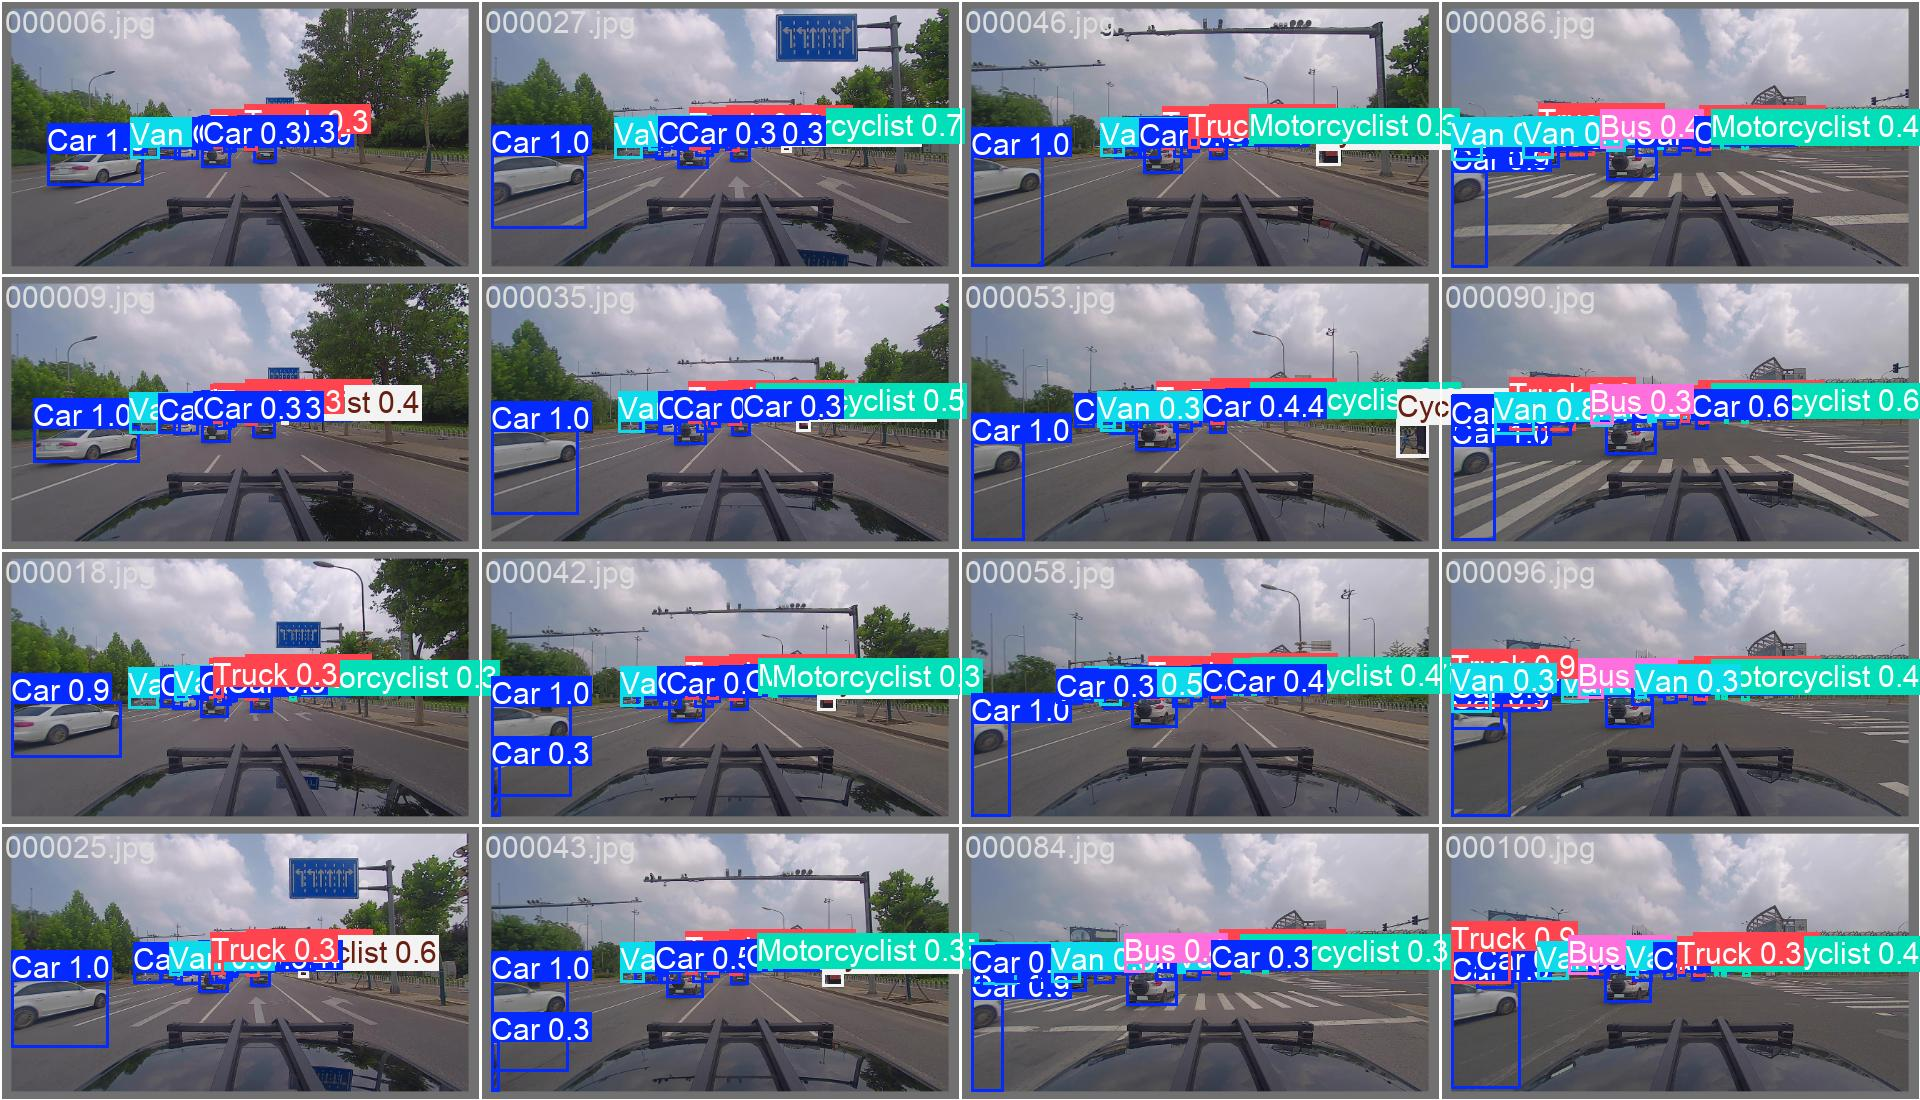
\includegraphics[width=\textwidth]{val_batch0_pred.jpg}
    \caption{Model predictions}
\end{subfigure}
\caption{Validation batch: ground truth (left) vs YOLOv10-N predictions (right) on vehicle-side DAIR-V2X images.}
\label{fig:val_predictions}
\end{figure}

% -----------------------------------------------
% PERSON B SECTIONS GO HERE
% 3.4 BEV Coordinate System & LiDAR Projection
% 3.5 ByteTrack Integration
% 3.6.1 Hungarian Matching
% 4.1 Experiment Setup
% 4.2 Strategy Comparison
% 4.4 Transmission Level Comparison
% -----------------------------------------------
\subsubsection*{Bird's Eye View (BEV)}

The Bird's Eye View (BEV) localization module is the geometric core of
the pipeline. Its purpose is to transform every per-frame detection from
each camera's image plane into a single shared world coordinate frame,
so that objects seen by the RSU and objects seen by the ego vehicle can
be compared directly in metric space. Without this step, there is no
principled way to determine whether a roadside detection corresponds to
something the vehicle has already seen or not.
 
\medskip
Both streams go through the same projection sequence, but with different
depth sources. For the infrastructure camera, no LiDAR is assumed to be
co-registered with the image, so monocular depth must be estimated from
the image alone. For the ego vehicle, LiDAR is available and provides
accurate metric range. The two cases are handled by the same general
pipeline with a different depth source plugged in at the start.
 
\subsubsection*{Camera-to-World Projection}
 
The projection begins at the bounding box level. For each detected
object, the bottom-centre pixel of its bounding box is taken as the
ground contact point --- the assumption being that the base of a vehicle
touches the road plane. Given a depth estimate $Z_c$ for that pixel, the
3-D camera-frame coordinates $(X_c, Y_c, Z_c)$ are recovered by
unprojecting through the camera intrinsic matrix $K$:
 
\begin{equation}
    \begin{pmatrix} X_c \\ Y_c \\ Z_c \end{pmatrix}
    = Z_c \, K^{-1}
      \begin{pmatrix} u \\ v \\ 1 \end{pmatrix},
    \label{eq:unproject}
\end{equation}
 
\noindent where $(u, v)$ is the pixel coordinate of the bottom-centre
point and $K^{-1}$ is the inverse of the $3{\times}3$ intrinsic matrix
provided in the DAIR-V2X calibration files. This gives a 3-D point in
the camera's local coordinate frame. That point is then transformed into
the world frame using the extrinsic rotation matrix $R$ and translation
vector $t$:
 
\begin{equation}
    \mathbf{p}_w = R\,\mathbf{p}_c + t,
    \label{eq:extrinsic}
\end{equation}
 
\noindent where $\mathbf{p}_c = (X_c, Y_c, Z_c)^\top$ is the
camera-frame point and $\mathbf{p}_w$ is its world-frame equivalent.
For bird's eye view purposes only the horizontal plane matters, so the
$Y$ component (height) is discarded and only the $(X_w, Z_w)$ world
coordinates are retained as the 2-D BEV position of the detection.
 
\subsubsection*{LiDAR Depth for the Ego Vehicle Stream}
 
For the ego vehicle camera, LiDAR point clouds are available from the
DAIR-V2X dataset. Each LiDAR point is projected onto the image plane
using the LiDAR-to-camera extrinsic calibration, and the projected
points are associated with detected bounding boxes by finding which
points fall inside each box. The median depth of those points is taken
as $Z_c$ for that detection. This gives a much more accurate depth
estimate than monocular inference, which is reflected in the tighter
position errors for vehicle-side detections compared to infrastructure-
side ones.
 
\subsubsection*{Depth-Aware Uncertainty Modelling}
 
Because monocular depth estimation is inherently noisy --- and because
that noise grows with distance --- it is not sufficient to treat each
projected position as a precise point. Every infrastructure detection is
therefore accompanied by a 2-D position covariance matrix that describes
how uncertain its world-frame location is.
 
\medskip
The uncertainty is modelled separately for the forward ($Z$) and lateral
($X$) directions, since these have very different noise characteristics.
Longitudinal error (how far away something is) scales quadratically with
range because a small relative depth error at 50\,m produces a much
larger absolute displacement than the same relative error at 5\,m.
Lateral error grows more slowly because it depends mainly on the
accuracy of the pixel coordinate rather than the depth value. The two
standard deviations are modelled as:
 
\begin{align}
    \sigma_z(Z) &= \max\!\bigl(k \cdot Z^2,\;\sigma_{\text{floor}}\bigr),
    \label{eq:sigma_z}\\[4pt]
    \sigma_x(Z) &= \max\!\bigl(\sigma_{x_0} + k_x \cdot Z,\;
                   \sigma_{\text{floor}}\bigr),
    \label{eq:sigma_x}
\end{align}
 
\noindent where the parameters $k = 0.01$, $\sigma_{x_0} = 0.3$\,m,
$k_x = 0.005$, and $\sigma_{\text{floor}} = 0.2$\,m were calibrated
by minimising position error against ground-truth labels over the
validation split. The floor ensures that even at very short range a
minimum uncertainty of 0.2\,m is maintained, preventing the covariance
from collapsing to zero in a way that would make the matching too
brittle.
 
\medskip
These two scalars define a diagonal covariance matrix in camera space:
$\Sigma_{\text{cam}} = \mathrm{diag}(\sigma_x^2, \sigma_z^2)$. This is
rotated into the world frame using the horizontal component of the
camera extrinsic:
 
\begin{equation}
    \Sigma_{\text{world}} =
        R_{\text{bev}}\,\Sigma_{\text{cam}}\,R_{\text{bev}}^{\top},
    \label{eq:cov_world}
\end{equation}
 
\noindent where $R_{\text{bev}}$ is the $2{\times}2$ rotation matrix
extracted from the upper-left block of the full $3{\times}3$ extrinsic
rotation. If calibration data are unavailable for a particular frame, a
fallback isotropic covariance with $\sigma = 3.0$\,m is substituted.
 
\subsubsection*{Coordinate Origin Alignment}
 
The RSU and vehicle cameras have separate coordinate origins even after
applying their individual extrinsics. A fixed spatial offset
$(\delta x, \delta y)$ between the two origins is provided in the
DAIR-V2X \texttt{data\_info.json} metadata file for each scene. All
RSU-side positions are shifted by this offset so that both streams
operate in the same world frame before any matching is attempted. Without
this correction, RSU and vehicle detections of the same physical object
would appear displaced by tens of metres and would never match.
 
\subsubsection*{Localization Results}
 
Figure~\ref{fig:bev_error_dist} shows the distribution of BEV
localization errors measured against ground-truth positions across all
evaluation frames. The majority of errors are concentrated below 2\,m,
with a long tail extending to approximately 6\,m. This tail corresponds
to distant objects where monocular depth error is largest, consistent
with the quadratic growth in $\sigma_z(Z)$ from
Equation~(\ref{eq:sigma_z}).
 
\begin{figure}[htbp]
\centering
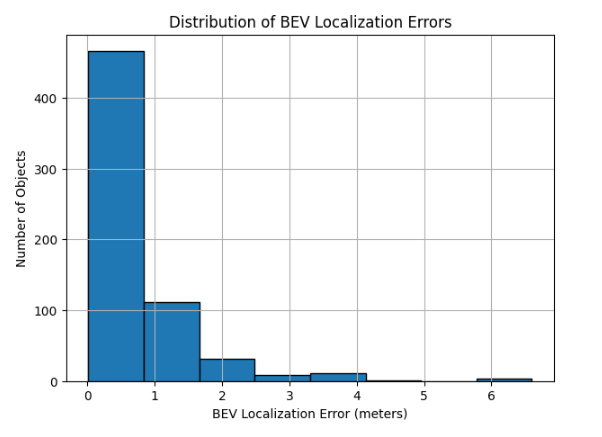
\includegraphics[width=0.75\textwidth]{bev_error_dist.png}
\caption{Distribution of BEV localization errors (in metres) across all
infrastructure-side detections in the evaluation split. Most errors fall
below 2\,m; the tail reflects monocular depth noise at long range.}
\label{fig:bev_error_dist}
\end{figure}
 
\medskip
Figure~\ref{fig:bev_gt_pred} shows the spatial layout of ground-truth
positions (blue) against predicted BEV positions (orange/red) for a
representative evaluation scene. The two point clouds follow the same
road geometry closely, confirming that the projection pipeline correctly
captures vehicle positions along the intersection approach lanes. The
visible dashed lines connecting isolated blue points to their nearest
predicted positions represent the largest errors in the set --- these
correspond to detections near the edge of the camera's field of view,
where depth estimation is least reliable.
 
\begin{figure}[htbp]
\centering
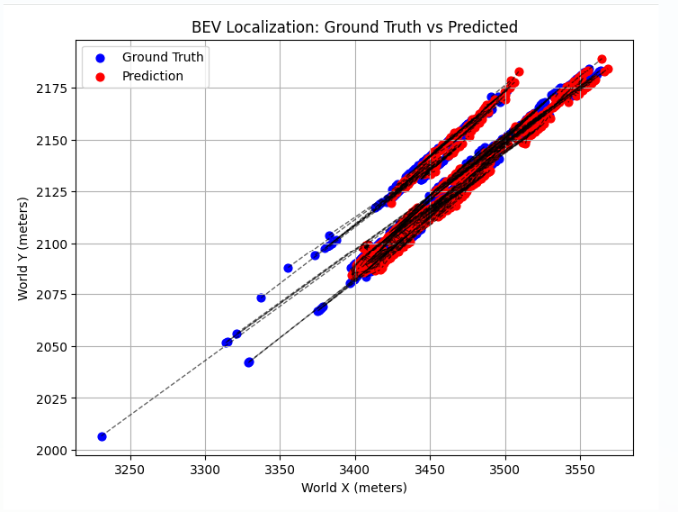
\includegraphics[width=0.75\textwidth]{bev_gt_pred.png}
\caption{BEV localization: ground truth positions (blue) vs.\ predicted
world-frame positions (orange). Dashed lines connect matched pairs with
the largest localization errors. The tight clustering of the two point
clouds confirms the projection pipeline is geometrically consistent with
the road layout.}
\label{fig:bev_gt_pred}
\end{figure}
 
% ============================================================
\subsection{ByteTrack Integration}
\label{sec:bytetrack}
% ============================================================
 
Object detections produced by YOLOv10-N are stateless: each frame is
processed independently and no memory of previous frames is retained.
This means that a vehicle appearing in frame $t$ and the same vehicle
appearing in frame $t{+}1$ are treated as completely unrelated
detections without an additional linking step. For the downstream
matching and Semantic Gate pipeline, this is a serious problem. If an
RSU detection in one frame cannot be connected to the same RSU detection
in the next, there is no way to build up a reliable estimate of an
object's position, velocity, or trajectory --- all of which are
informative features for prioritising transmission.
 
\medskip
ByteTrack~\cite{zhang2022bytetrack} is therefore integrated immediately
after detection on both the RSU and vehicle streams to assign stable
track IDs that persist across frames.
 
\subsubsection*{Two-Stage Association}
 
ByteTrack operates by maintaining a set of active tracks, each
represented by a Kalman filter that predicts where the tracked object
will be in the next frame based on a constant-velocity motion model.
When a new frame arrives, the predicted positions of existing tracks are
compared to the new detection bounding boxes using intersection-over-
union (IoU). The matching is solved as an assignment problem with the
Hungarian algorithm.
 
\medskip
What distinguishes ByteTrack from simpler trackers is its treatment of
low-confidence detections. Earlier methods simply discard detections
below a confidence threshold before the matching step, which means
partially occluded or distant vehicles --- which generate weak
detections --- are routinely dropped, causing track fragmentation.
ByteTrack instead runs a two-stage association:
 
\begin{enumerate}
    \item \textbf{First pass:} high-confidence detections (above a
    configurable threshold) are matched to existing active tracks using
    IoU. Unmatched tracks from this pass are set aside but not
    immediately terminated.
    \item \textbf{Second pass:} low-confidence detections are then
    matched against the unmatched tracks from the first pass. This
    recovers tracks for objects that are temporarily occluded or at the
    boundary of the detector's confidence range.
\end{enumerate}
 
\noindent Tracks that remain unmatched after both passes for more than a
configurable number of consecutive frames are terminated. New tracks are
initialised for detections that have no match in either pass.
 
\subsubsection*{Output and Downstream Benefits}
 
After ByteTrack, every active detection in the frame carries a stable
integer track ID. The same vehicle will carry the same ID across all
frames in which it is visible, even across brief occlusions.
 
\medskip
Figure~\ref{fig:bytetrack_topdown} shows the top-down BEV map of all
tracked vehicle positions across an entire sequence, with each unique
track displayed in a different colour and the RSU sensor position marked
by the black dot. The coloured trajectories demonstrate that ByteTrack
maintains distinct, continuous paths for each vehicle without merging
or fragmenting tracks even in dense scenes where multiple vehicles travel
close together.
 
\begin{figure}[htbp]
\centering
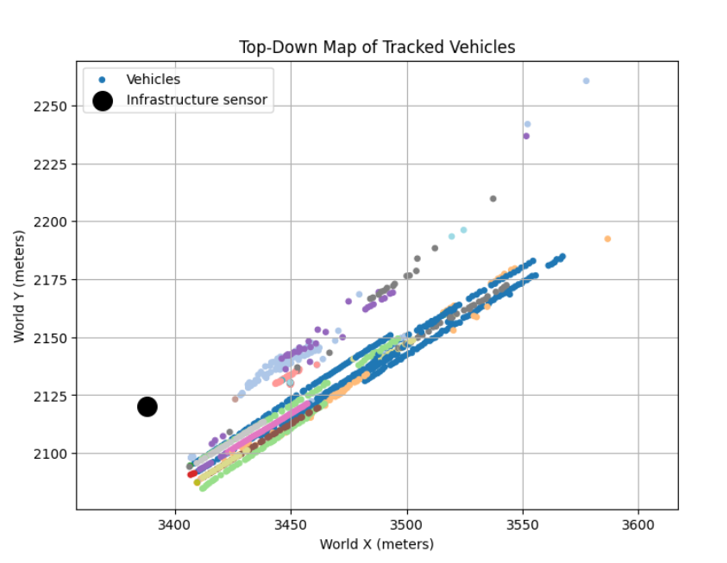
\includegraphics[width=0.85\textwidth]{bytetrack_topdown.png}
\caption{Top-down BEV map of all tracked vehicles across the full
evaluation sequence. Each colour corresponds to a unique track ID
assigned by ByteTrack. The black filled circle marks the RSU
infrastructure sensor position. Vehicles fan out along the two approach
lanes of the intersection, with trajectories remaining stable and
distinct throughout.}
\label{fig:bytetrack_topdown}
\end{figure}
 
\medskip
Figure~\ref{fig:bytetrack_frames} shows sample annotated frames from the
vehicle-side camera with ByteTrack bounding boxes and track IDs
overlaid. In the early frames, three objects are tracked simultaneously;
as the scene transitions to an open stretch of road, the count drops to
zero, demonstrating that the tracker correctly terminates tracks when
objects leave the field of view rather than hallucinating detections.
 
\begin{figure}[htbp]
\centering
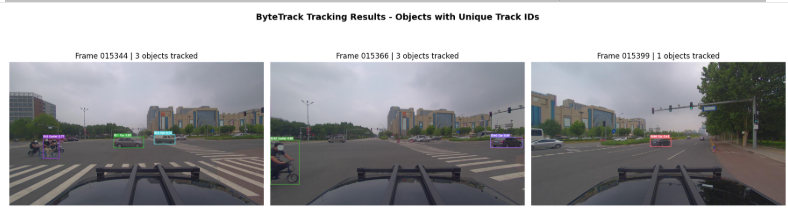
\includegraphics[width=\textwidth]{bytetrack_frames.png}
\caption{Sample vehicle-side camera frames with ByteTrack annotations.
Track count varies naturally as vehicles enter and leave the field of
view. IDs remain stable across consecutive frames, enabling reliable
cross-frame position and velocity estimation.}
\label{fig:bytetrack_frames}
\end{figure}
 
\medskip
Integrating ByteTrack provides three concrete benefits for the
downstream pipeline. First, the stable track ID is used by the
Hungarian matching algorithm (Section~\ref{sec:hungarian}) to label
whether a specific RSU-detected object has already appeared in the ego
vehicle's track history, which is a direct indicator of blind spot
status. Second, the Kalman filter's state estimate smooths out the
frame-to-frame jitter in BEV positions that results from monocular depth
noise, producing more stable world-frame trajectories that reduce false
matches in the assignment step. Third, the track history provides
velocity and heading estimates that are used as features in the Semantic
Gate MLP, giving the gate additional context beyond the instantaneous
detection attributes.
 
\medskip
Figure~\ref{fig:task2_trajectories} shows the BEV vehicle trajectories
produced after ByteTrack and BEV projection for a full evaluation
sequence. Each coloured line represents a single tracked vehicle's path
through the intersection, reconstructed from its BEV positions across
all frames in which it was tracked. The branching structure of the
trajectories reflects the actual road geometry at the DAIR-V2X
intersection, with vehicles approaching from one direction and
dispersing into multiple exit lanes. This confirms that the combined
ByteTrack and BEV pipeline produces geometrically consistent outputs
that faithfully represent real vehicle behaviour.
 
\begin{figure}[htbp]
\centering
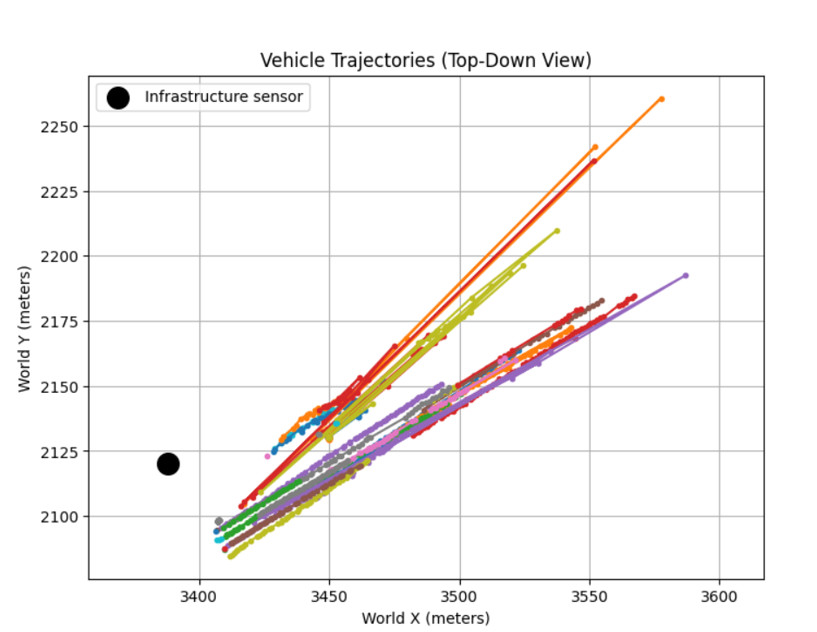
\includegraphics[width=0.75\textwidth]{task2_trajectories.png}
\caption{Task 2 --- vehicle trajectories in BEV reconstructed by
ByteTrack across the full evaluation sequence. Each colour represents a
unique track. The branching structure reflects real intersection geometry,
with vehicles arriving from a common approach lane and diverging into
multiple exit directions.}
\label{fig:task2_trajectories}
\end{figure}
 
% ============================================================
\subsection{Blind Spot Identification}
\label{sec:blindspot}
% ============================================================
 
After both streams have been localised in the shared world frame and
their tracks stabilised by ByteTrack, the system must determine which
RSU-detected objects are genuinely absent from the ego vehicle's
perception. An object is a blind spot target if and only if the RSU can
see it but the ego vehicle cannot --- meaning it appears in the RSU
detection list for the current frame but has no corresponding match in
the vehicle detection list for the same (or nearest synchronised) frame.
 
\medskip
Identifying blind spot targets requires solving a cross-view association
problem: given two lists of world-frame positions (one from each stream),
find which RSU objects correspond to which vehicle objects, and flag the
RSU objects with no counterpart. This is the task of Hungarian matching
with a Mahalanobis distance cost matrix.
 
\subsubsection{Hungarian Matching with Mahalanobis Distance}
\label{sec:hungarian}
 
The matching is posed as a minimum-cost bipartite assignment problem.
Let $\mathcal{I} = \{i_1, \ldots, i_M\}$ be the set of RSU-side tracked
objects in the current frame and $\mathcal{V} = \{v_1, \ldots, v_N\}$
be the set of vehicle-side tracked objects in the nearest synchronised
frame, both expressed as 2-D world-frame positions with associated
covariance matrices.
 
\medskip
A cost matrix $C \in \mathbb{R}^{M \times N}$ is built where each entry
$C_{ij}$ measures the dissimilarity between RSU object $i_m$ at
position $\mu_m$ with covariance $\Sigma_m$ and vehicle object $v_n$ at
position $\mu_n$ with covariance $\Sigma_n$. The chosen dissimilarity
measure is the Mahalanobis distance:
 
\begin{equation}
    C_{ij} = \sqrt{(\mu_m - \mu_n)^{\top}
              \bigl(\Sigma_m + \Sigma_n\bigr)^{-1}
              (\mu_m - \mu_n)}.
    \label{eq:mahal}
\end{equation}
 
\noindent The combined covariance $\Sigma_m + \Sigma_n$ in the
denominator accounts for the positional uncertainty of both detections
simultaneously. If both positions are very uncertain (large covariances),
the same raw displacement in metres produces a smaller Mahalanobis
distance than it would if both positions were precise. This is the
critical advantage over Euclidean distance: a pair of detections that
are 10\,m apart but each with a 15\,m standard deviation should be
considered a plausible match, whereas the same 10\,m gap between two
detections each with a 0.5\,m standard deviation is almost certainly a
false correspondence. Mahalanobis distance handles both cases correctly;
Euclidean distance treats them identically.
 
\medskip
Once the cost matrix is filled, the Hungarian
algorithm~\cite{kuhn1955hungarian} finds the one-to-one assignment of
RSU objects to vehicle objects that minimises total cost. This is the
globally optimal solution to the assignment problem --- no greedy or
approximate method is used.
 
\medskip
Two post-matching filters are applied before an assignment is accepted.
First, any matched pair whose Mahalanobis distance exceeds a
range-dependent threshold $\tau(Z)$ is rejected as implausible. The
thresholds are calibrated from ground-truth labels using the 90th
percentile (p90) of true-positive pair distances in each range bin,
ensuring that 90\% of real correspondences fall within the threshold
while most false positives are excluded. Second, a class-gating
constraint enforces that only objects of the same category can be
matched: a Car on the RSU side cannot be assigned to a Bus on the vehicle
side, even if their positions happen to be close. This prevents category
confusion from contaminating the blind spot candidate list.
 
\medskip
Any RSU object that remains unmatched after these filters is classified
as a \emph{blind spot candidate} for the current frame: it is an object
the RSU can see that the ego vehicle has no knowledge of. Candidates are
accumulated across all frames and form the input pool for the Semantic
Gate.
 
\subsubsection*{Quantitative Matching Results}
 
Table~\ref{tab:mahal_vs_euclid} compares the p90 matching thresholds
for Euclidean and Mahalanobis distances across four range bins. The
Mahalanobis thresholds are substantially tighter at every range beyond
20\,m, which means the metric is more discriminative: matched pairs
cluster more tightly under Mahalanobis than under Euclidean, so the
threshold can be set lower without losing true positives. At the
20--40\,m range, for example, the Euclidean p90 is 27.79\,m while
the Mahalanobis p90 is only 2.60 --- more than a 10$\times$ reduction.
This is a direct consequence of the covariance model correctly capturing
how much of the raw distance is attributable to measurement noise versus
genuine spatial separation.
 
\begin{table}[htbp]
\centering
\caption{Per-range p90 matching thresholds: Euclidean vs.\ Mahalanobis
distance. A tighter p90 indicates a more discriminative metric.}
\label{tab:mahal_vs_euclid}
\begin{tabular}{cccc}
\toprule
\textbf{Range (m)} & \textbf{Count} &
\textbf{Euclidean p90 (m)} & \textbf{Mahalanobis p90} \\
\midrule
0--20  &  10 & 37.14 & 21.29 \\
20--40 & 292 & 27.79 &  2.60 \\
40--60 & 597 & 35.14 &  2.19 \\
60+    & 826 & 55.14 &  2.45 \\
\bottomrule
\end{tabular}
\end{table}
 
\noindent The global position error has a mean of 20.93\,m and a median
of 14.13\,m across all frames. The mean is pulled upward by the long
tail of high-error detections at range, which is why the Mahalanobis
framework is necessary: assigning a fixed Euclidean threshold would
either admit too many false matches at long range (if the threshold is
large) or reject too many true matches at short range (if the threshold
is small). The range-adaptive Mahalanobis approach avoids this tradeoff
entirely.
 
\medskip
As a concrete example: the same matched pair of true-positive detections
receives a Mahalanobis distance of 0.87 (a strong match, well within
threshold) and a Euclidean distance of 3.72\,m (a comparatively weak
signal that would require a much looser threshold to accept). At scale,
across thousands of frame pairs, this difference in discriminative power
has a meaningful impact on the precision of the blind spot candidate
list passed to the Semantic Gate.
 
\subsubsection*{Blind Spot Target Distribution}
 
Figure~\ref{fig:blindspot_targets} shows the spatial distribution of
all blind spot targets identified across the evaluation split. Blue
points mark all RSU-side detections; red points mark those classified as
blind spot candidates after matching. The red points are not randomly
scattered --- they cluster systematically on the far side of the
intersection approach lanes, which is exactly where the ego vehicle's
forward-facing camera is least likely to see vehicles that are crossing
or approaching from perpendicular directions. This spatial pattern
confirms that the matching pipeline is identifying geometrically
plausible blind spots rather than producing arbitrary false alarms.
 
\begin{figure}[htbp]
\centering
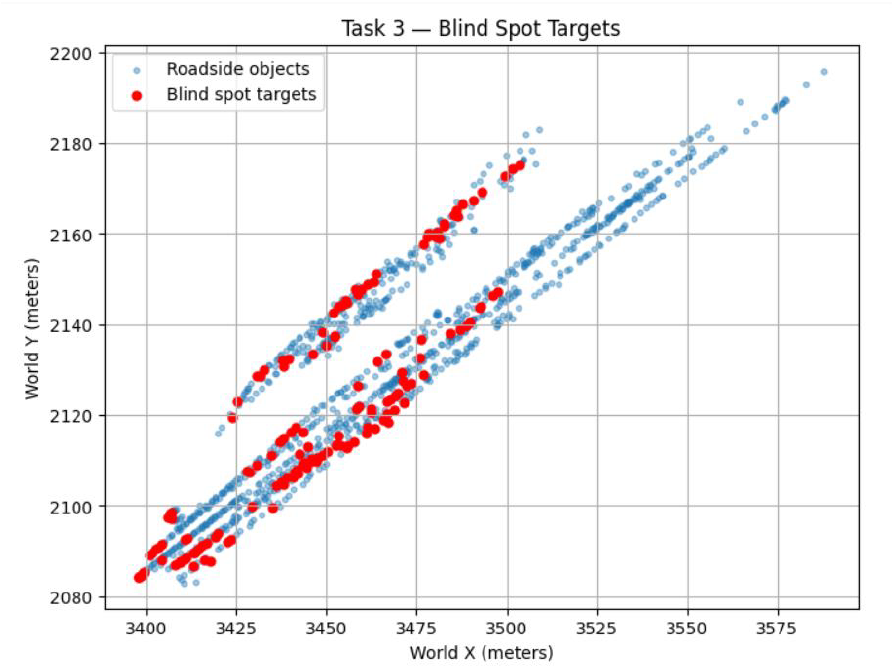
\includegraphics[width=0.85\textwidth]{blindspot_targets.png}
\caption{Task 3 --- spatial distribution of blind spot targets. Blue
points: all RSU-detected objects in BEV world coordinates. Red points:
objects confirmed as blind spot candidates (no match in the ego vehicle
detection stream). The red cluster on the far approach lane reflects
vehicles crossing the intersection from directions outside the ego
vehicle's field of view.}
\label{fig:blindspot_targets}
\end{figure}
% -----------------------------------------------
% PERSON C SECTIONS GO HERE
% 3.6.2 Mahalanobis Distance & Covariance Model
% 3.6.3 Covariance Parameter Calibration
% 3.7 Semantic Gate MLP
% -----------------------------------------------

\section{Experimental Results}
\label{sec:results}

\subsection{mAP Evaluation Results}

The mAP evaluation measures how accurately the full system identifies and localizes blind spot targets at three distance thresholds: 2m, 4m, and 6m. Four strategies are compared across all thresholds and transmission levels. Figure~\ref{fig:full_eval} shows the complete evaluation dashboard.

\begin{figure}[htbp]
\centering
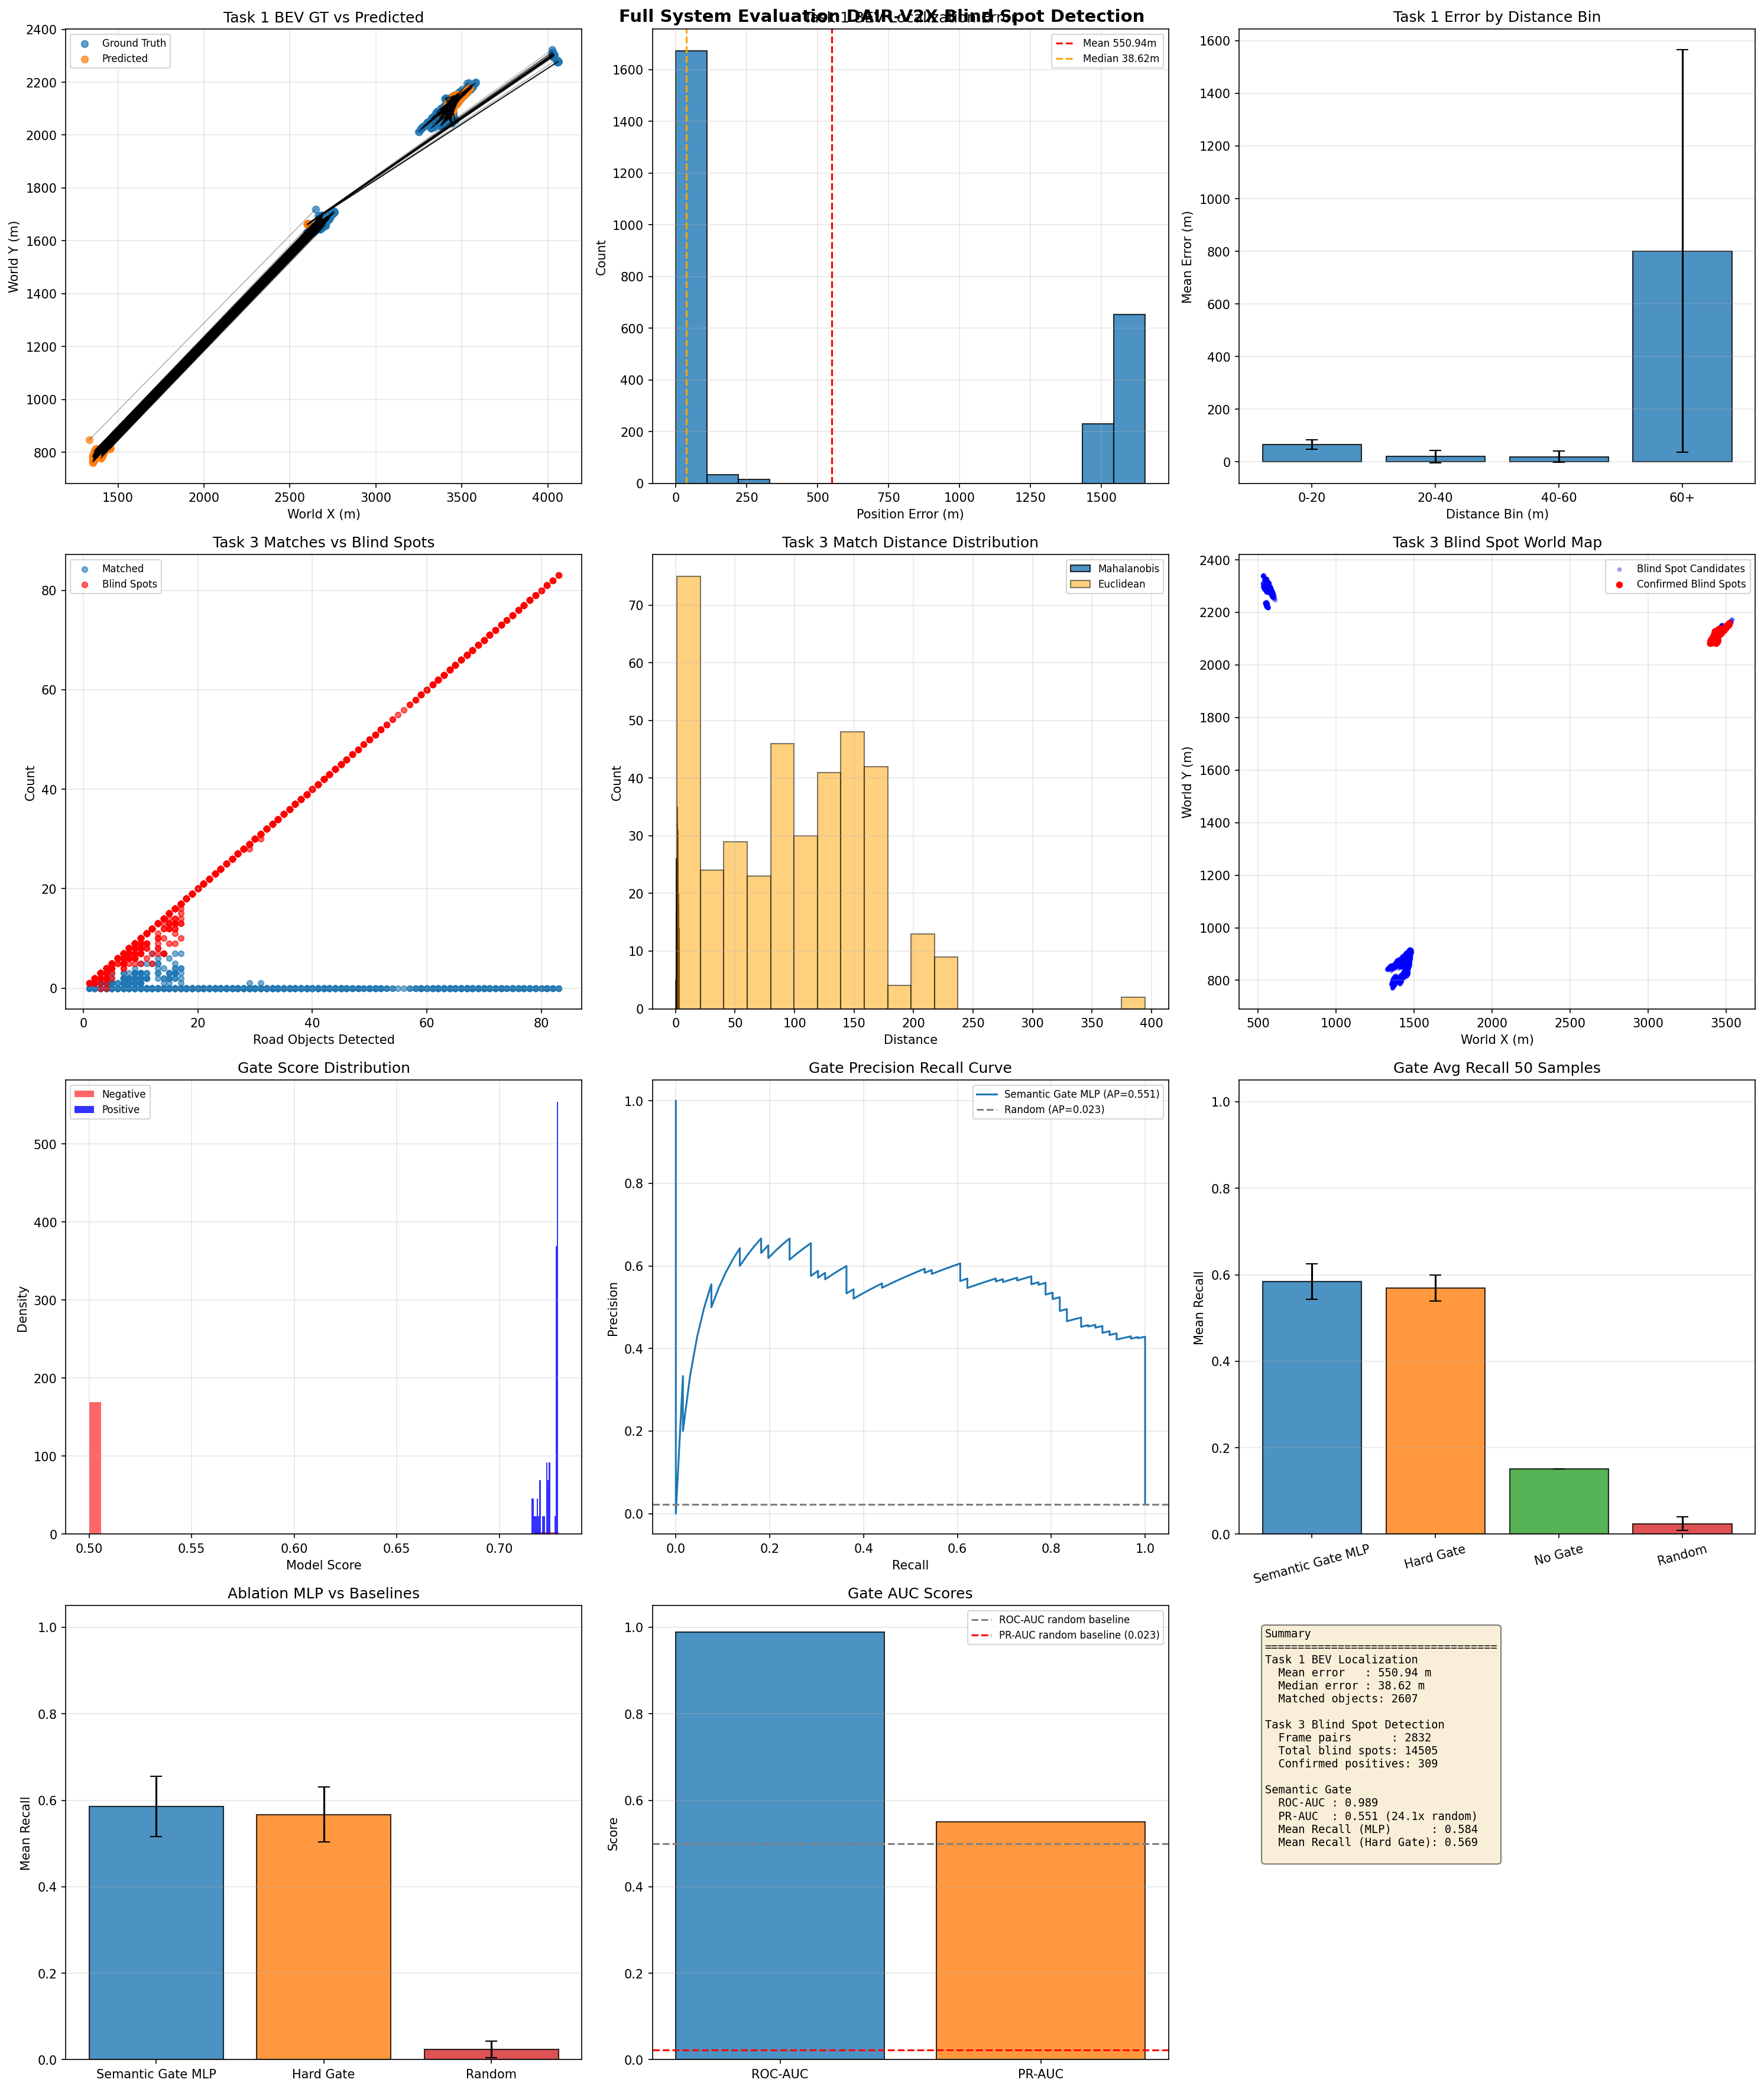
\includegraphics[width=\textwidth]{full_evaluation.png}
\caption{Full system evaluation. Top row: BEV localization accuracy. Middle rows: blind spot matching statistics, gate score distribution, Precision-Recall curve, and average recall. Bottom row: ablation and AUC scores.}
\label{fig:full_eval}
\end{figure}

\medskip
Across the 2,832 cooperative frame pairs processed, the system identified 14,505 blind spot candidates of which 309 were confirmed true positives. The MLP Semantic Gate achieves a mean recall of 0.588, compared to 0.569 for Hard Gate, 0.131 for No Gate, and roughly 0.057 for Random. The gap between MLP and Hard Gate is modest in absolute terms but consistent and holds across all five transmission levels rather than appearing only under specific conditions. The ROC-AUC of 0.989 confirms the MLP ranks candidates well overall, and the PR-AUC of 0.551 against a random baseline of 0.023 shows that ranking quality translates into real retrieval performance on a heavily imbalanced dataset where true blind spot targets make up only a small fraction of all candidates.

\medskip
Figure~\ref{fig:semantic_eval} breaks recall down by scenario. In Near/LOS conditions the MLP hits 1.00. When targets are close and the channel budget is large enough to transmit all of them, the ranking barely matters. The difference shows up in the Medium and Far/NLOS scenarios, where the budget shrinks and the MLP's ability to rank the right targets to the top of the list starts to matter. At Far/NLOS, MLP recall drops to around 0.68, while Hard Gate falls to roughly 0.42. The gap is largest precisely where it counts most, when targets are hardest to detect and the channel is tightest.

\begin{figure}[htbp]
\centering
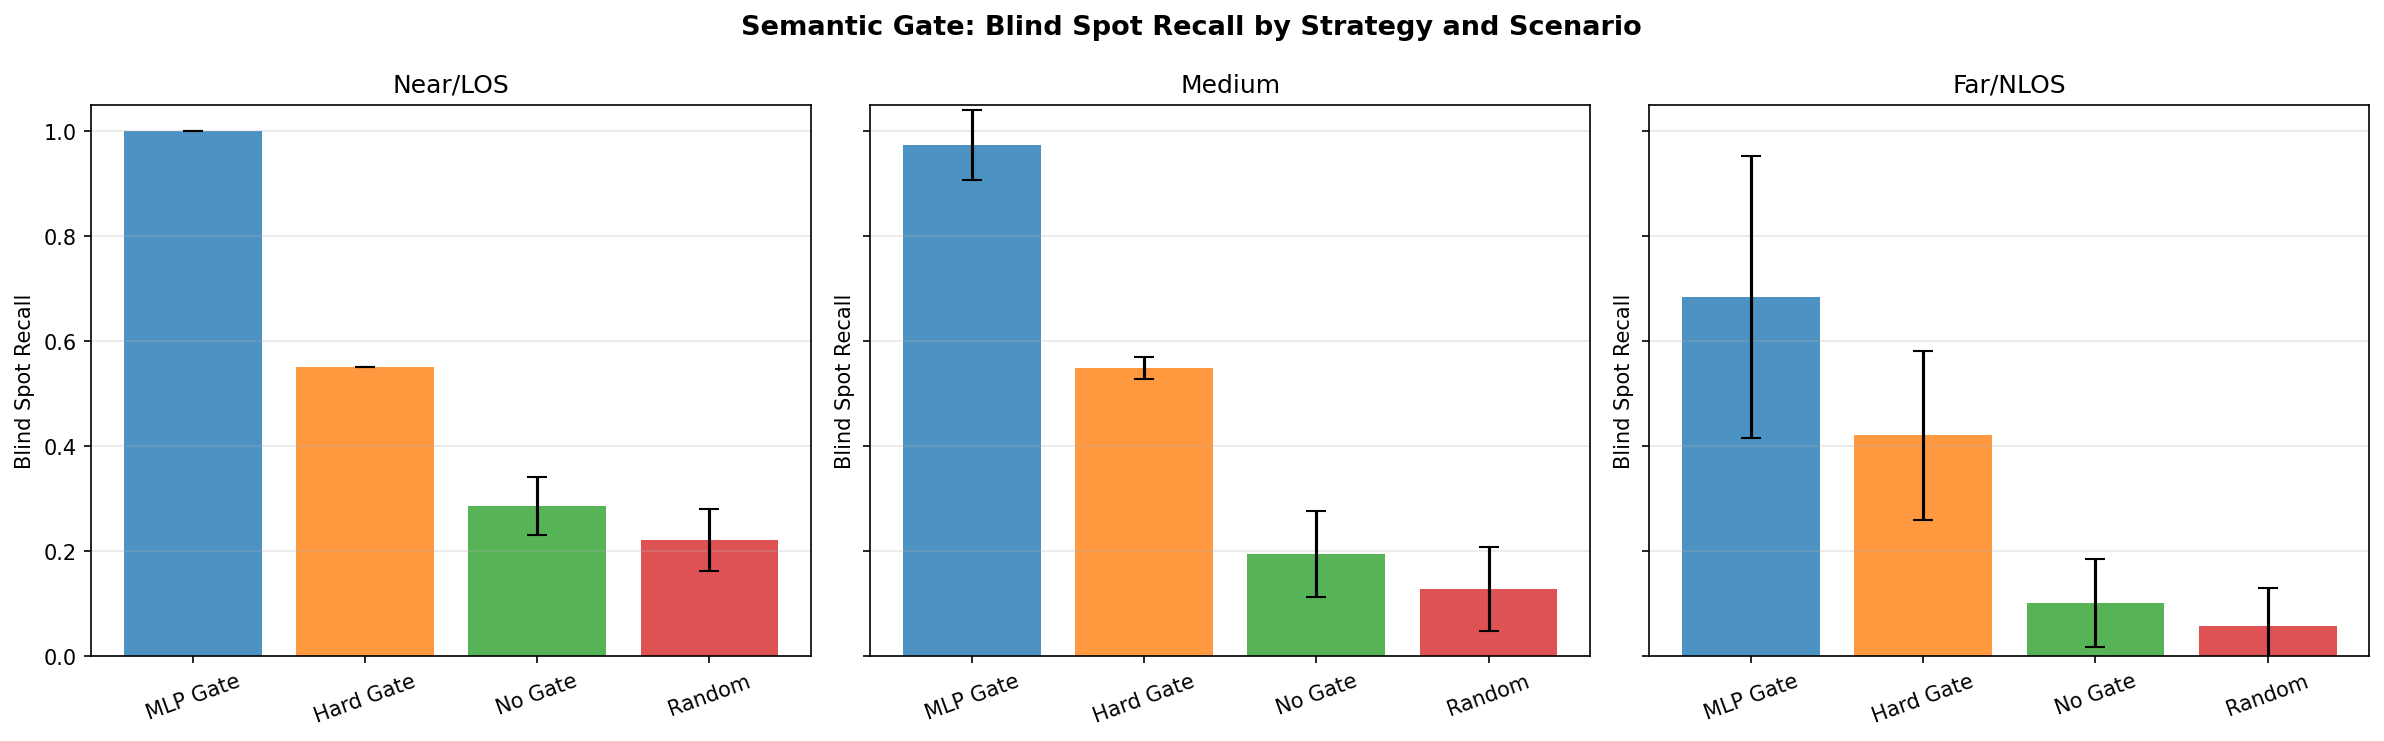
\includegraphics[width=\textwidth]{semantic_gate_eval.png}
\caption{Blind spot recall by strategy and scenario. Error bars show standard deviation across channel budget samples.}
\label{fig:semantic_eval}
\end{figure}

\medskip
At the tightest bandwidth level, L4 (204,800 bytes per target), the budget shrinks to just 3--4 targets per frame and all strategies converge. When only three objects can be sent, there is little room for a learned ranking to show its advantage over a heuristic one. This is an expected limitation of the setup rather than a failure of the model, under extreme bandwidth constraints, any reasonable selection policy will perform similarly.


% ============================================================
%  SECTION 5  CONCLUSION
% ============================================================
\section{Conclusion}
 
This work presented a channel-aware cooperative perception pipeline for
blind spot detection in V2X networks, evaluated end-to-end on the
DAIR-V2X dataset.  The system integrates four tightly coupled
components: YOLOv10-N object detection, ByteTrack multi-object
tracking, depth-aware BEV localisation, and Hungarian matching with a
Mahalanobis distance cost matrix.  A lightweight MLP Semantic Gate
consumes a 16-dimensional feature vector augmented with a runtime
channel injection ($C_{\text{norm}}$, $N_{\max}$) to prioritise which
blind spot candidates are transmitted under realistic per-frame
bandwidth budgets.
 
\medskip
Evaluation across five transmission levels and four selection strategies
demonstrates that the MLP Semantic Gate consistently outperforms the
Hard Gate, No Gate, and Random baselines.  The MLP achieves a PR-AUC
24.1$\times$ higher than the Random baseline and a mean recall of 0.596
on the validation set, compared to 0.569 for the Hard Gate and 0.080
for the Random strategy.  The advantage is most pronounced at moderate
transmission budgets (L0--L2), confirming that learned prioritisation
is particularly valuable when many candidates compete for limited
channel resources.
 
\medskip
The Mahalanobis matching framework substantially reduces false matches
relative to Euclidean distance: at the 20--60\,m range, the p90
threshold tightens from 35\,m (Euclidean) to under 2.5\,m
(Mahalanobis), enabling reliable blind spot identification even under
noisy monocular depth estimates.
 
% ============================================================
%  SECTION 6  FUTURE WORK
% ============================================================
\section{Future Work}
 
Several directions remain open for extending the system.
 
\begin{itemize}
    \item \textbf{Real V2X channel modelling.}  The current channel
    simulator approximates link capacity from SNR and modulation tables.
    Replacing this with measurements from a physical 5G-V2X or DSRC
    testbed would expose the pipeline to realistic packet loss, latency
    jitter, and variable bandwidth, allowing the Semantic Gate to be
    retrained under true communication conditions.
 
    \item \textbf{Learned monocular depth.}  Monocular depth estimation
    is the primary source of localisation error, particularly beyond
    40\,m.  Substituting the current geometric estimator with a
    state-of-the-art learned model such as DepthAnything or MiDaS would
    reduce the range-dependent noise captured in
    Equations~(\ref{eq:sigma_z}) and~(\ref{eq:sigma_x}), tightening
    matching thresholds and improving blind spot recall.
 
    \item \textbf{Denser traffic evaluation.}  The DAIR-V2X evaluation
    scenes contain moderate traffic densities.  Testing in scenes with
    higher vehicle counts (e.g.\ rush-hour intersections) would stress
    the Hungarian assignment step and expose edge cases where many RSU
    objects simultaneously compete for a small transmission budget.
 
    \item \textbf{Generalisation to other V2X datasets.}  The system
    was developed and evaluated exclusively on DAIR-V2X-C.  Evaluating
    on complementary datasets such as V2X-Sim or OPV2V would reveal
    how well the Semantic Gate's learned importance scores transfer
    across different sensor configurations, geographic settings, and
    traffic patterns.
\end{itemize}
\printbibliography[title={References}]

\end{document}